\chapter{A Lagrangian perspective}
\label{lagrangian-perspective}

Tracing its origins to mechanics theories for solid continua, the
following formulation for biological growth is developed naturally in
terms of {\em material quantities} defined in the {\em reference
  configuration} of the tissue. During the course of this chapter, the
fundamental field equations of a continuum idealisation of tissues are
derived from general principles governing the behaviour of multiphase
mixtures. Specifically, Section~\ref{balance-laws} helps define the
system and formally introduces fundamental quantities characterising
it, before deriving the balance laws from fundamental
axioms. Section~\ref{kinematics-of-growth}, presents the kinematics
associated with finite deformation growth. A fundamental axiom of
thermodynamics, the entropy inequality, and its restriction on
functional forms of constitutive relationships is the subject of
Section~\ref{entropy-inequality}. The chapter concludes with novel
algorithmic considerations (Section~\ref{algorithmic-considerations})
which play an important role in the computational formulation
underlying the numerical experiments presented in
Chapter~\ref{numerical-simulations-1}.

\section{Balance laws for an open mixture}
\label{balance-laws}

The tissue of interest is idealised as an open subset of
$\mathbb{R}^3$ with a piecewise smooth boundary. At a reference
placement of the tissue, $\Omega_0$, points in the tissue are
identified by their reference positions, $\bX \in \Omega_0$. The
motion of the tissue is a sufficiently smooth bijective map $\Bvarphi:
\overline{\Omega}_0 \times [0,T] \rightarrow \mathbb{R}^3$, where
$\overline{\Omega}_0 := \Omega_0 \cup \partial\Omega_0$;
$\partial\Omega_0$ being the boundary of $\Omega_0$. At a typical time
$t \in [0,T]$, $\Bvarphi(\bX,t)$ maps a point $\bX$ to its current
position, $\bx$. In its current configuration, the tissue occupies a
region $\Omega_t = \Bvarphi_t (\Omega_0)$. These details are depicted
in Figure~\ref{continuum-potato-mass}. The deformation gradient $\bF
:= \partial \Bvarphi/ \partial\bX$ is the tangent map of $\Bvarphi$.

\begin{figure}
  \centering
  \psfrag{A}{$\bX$}
  \psfrag{F}{$\bx$}
  \psfrag{B}{\renewcommand{\baselinestretch}{1.5}$\Pi^\iota$}
  \psfrag{G}{$\pi^\iota$}
  \psfrag{E}{$\Bvarphi$}
  \psfrag{C}{$\Omega_0$}
  \psfrag{H}{$\Omega_t$}
  \psfrag{D}{$\bN\cdot\bM^\iota$}
  \psfrag{I}{$\bn\cdot\bm^\iota$}
  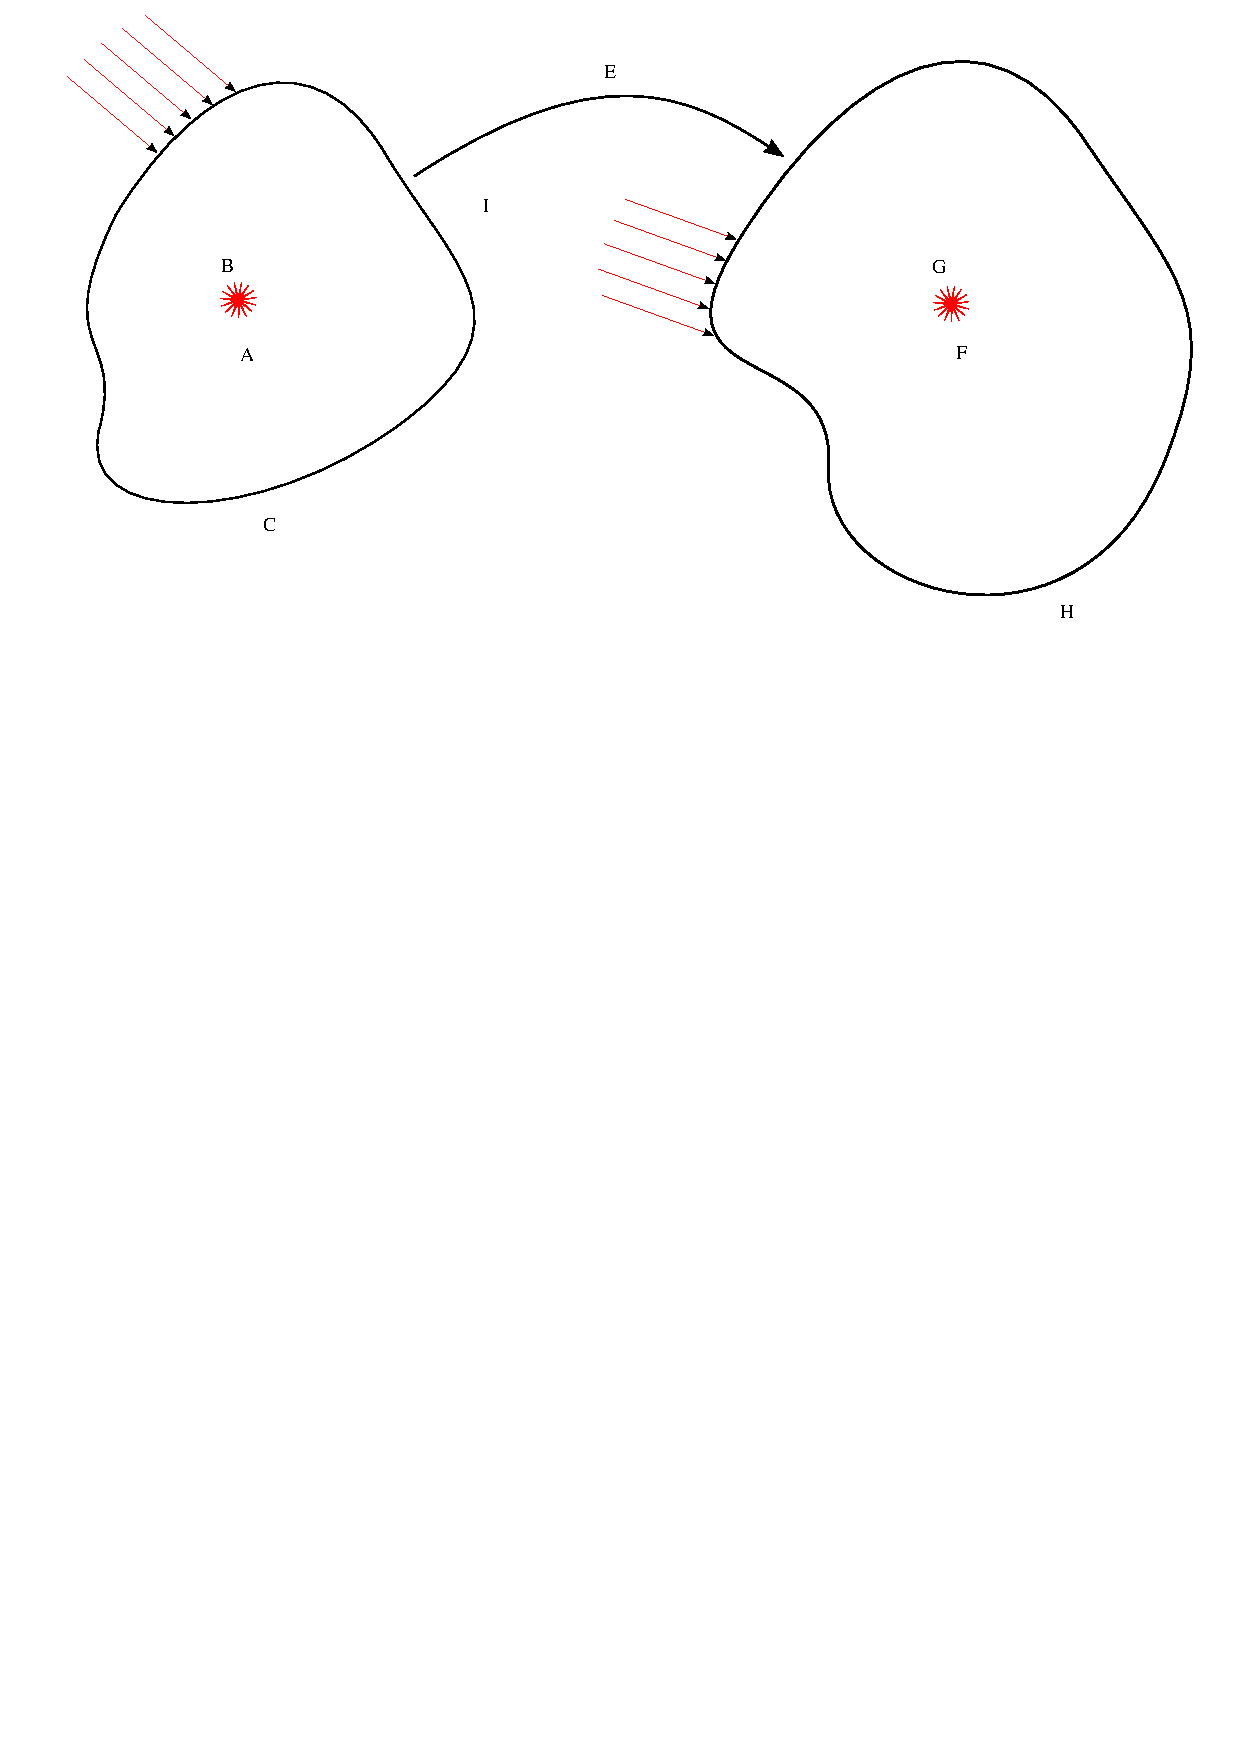
\includegraphics[width=0.8\textwidth]{images/elucidation/continuum-potato-mass}
  \caption{The tissue as a continuous medium with growing and
    diffusing species.} 
  \label{continuum-potato-mass}
\end{figure}

The tissue consists of numerous species, of which the following
groupings are of importance for the models: A solid species,
consisting of solid \emph{collagen fibrils} and
\emph{cells},\footnote{At this point, the solid species is not
  differentiated any further. This is a good approximation to the
  physiological setting for tendons, which are relatively acellular
  and whose dry mass consists of up to 75\% collagen
  \citep{Nordinetal:2001}. When modelling tumour growth in a later
  chapter (Section~\ref{tumour-growth}), where cell mechanics and
  migration are significant \citep{namyetal:04}, the solid phase is
  further distinguished.} denoted by $\mathrm{c}$, an extra-cellular
\emph{fluid} species, denoted by $\mathrm{f}$, consisting primarily of
water, and \emph{solute} species, consisting of precursors to
reactions, byproducts, nutrients, and other regulatory chemicals. A
generic solute will be denoted by $\mathrm{s}$. In the treatment that
follows, an arbitrary species will be denoted by $\iota$, where $\iota
= \mathrm{c,f,s}$.

The fundamental quantities of interest are mass concentrations,
$\rho_0^\iota(\bX,t)$. These are the masses of each species per unit
system volume in $\Omega_0$. Formally, these quantities can also be
thought of in terms of the maps $\rho_0^\iota: \overline{\Omega}_0
\times [0,T] \rightarrow \mathbb{R}$, upon which the formulation
imposes some smoothness requirements. By definition, the total {\em
  material density} of the tissue at a point is a summation of these
concentrations over all species $\sum\limits_{\iota}\rho_0^\iota =
\rho_0$.

The system is open with respect to mass. Other than the solid species,
$\mathrm{c}$, all phases have mass fluxes, $\bM^\iota$.\footnote{As
  previously mentioned, when modelling certain physiological processes
  such as tumour growth or wound healing, where migration of cells
  within the extra-cellular matrix is consequential, the solid phase
  is further differentiated and cell migration is modelled as mass
  transport.}  These are mass flow rates per unit cross-sectional area
in the reference configuration \emph{defined relative to the solid
  phase}. The species have mass sources (or sinks), $\Pi^\iota$. The
sources specify mass production rates per unit volume of the body in
its reference configuration, $\Omega_0$.

\subsection{Balance of mass}
\label{balance-of-mass}

As a result of mass transport (via the flux terms) and
inter-conversion of species (via the source/sink terms) introduced
above, the concentrations, $\rho_0^\iota$, change with time. Written
in integral form, the balance of mass for an arbitrary species over
$\Omega_0$ states

\begin{equation}
\underbrace{\frac{\mathrm{d}}{\mathrm{d}t} \int\limits_{\Omega_0}
  \rho_0^\iota (\bX,t)\mathrm{d}V}_{\text{Rate of change of mass}} =
\underbrace{\int\limits_{\Omega_0} \Pi^\iota
  (\bX,t)\mathrm{d}V}_{\text{Mass being created}}
-\underbrace{\int\limits_{\partial\Omega_0}\bM^\iota(\bX,t)\cdot\bN
  \mathrm{d}A}_{\text{Mass leaving the domain}},
\label{globalbalanceofmass}
\end{equation}

\noindent where $\bN$ is the unit outward normal to the boundary,
$\partial\Omega_0$.

Applying Gauss' divergence theorem (Appendix~\ref{gauss-divergence})
to the surface integral term, and localising the result (recalling
that since $\Omega_0$ is a fixed volume, the time derivative on the
first term can be simply moved into the integral), we arrive at the
following local form of the balance of mass for an arbitrary species
in the reference configuration,

\begin{equation}
\frac{\partial\rho_0^\iota}{\partial t} = \Pi^\iota -
\mathrm{DIV}[\bM^\iota],\;\forall\,\iota.
\label{localbalanceofmass}
\end{equation}

\noindent Here, $\mathrm{DIV[\bullet]}$ is the divergence operator in
the reference configuration. The functional forms of $\Pi^\iota$ are
abstractions of the underlying biochemistry, physiologically relevant
examples of which are discussed in
Section~\ref{nature-of-sources}. The fluxes, $\bM^\iota$, are
determined from the thermodynamically-motivated constitutive relations
described in
Section~\ref{fluid-flux-constitutive-relationships}. Recall that, in
particular, $\bM^{c} = \bzero$.

The sources, $\Pi^\iota$ for various species, satisfy a relation
$\sum\limits_\iota\Pi^\iota = 0$, which is derived as
follows. Firstly, summing Equation~(\ref{globalbalanceofmass}) over
all species leads to the law of mass balance for the system,

\begin{equation}
\frac{\mathrm{d}}{\mathrm{d}t} \sum\limits_\iota\int\limits_{\Omega_0}
\rho_0^\iota \mathrm{d}V = \sum\limits_\iota 
\int\limits_{\Omega_0} \Pi^\iota \mathrm{d}V
- \sum\limits_\iota \int\limits_{\partial\Omega_0}\bM^\iota\cdot\bN
\mathrm{d}A. 
\label{masssummation}
\end{equation}

\noindent An alternate way of arriving at the mass balance equation
for the system is to envision an external observer accounting only for
the fluxes at the boundary, not aware of any processes internal to the
system. Following this viewpoint, we neglect the interconversion terms
(sources/sinks) which exist within the system, and arrive at,

\begin{equation}
\frac{\mathrm{d}}{\mathrm{d}t}\sum\limits_\iota
\int\limits_{\Omega_0}\rho_0^\iota \ \mathrm{d}V =
-\sum\limits_\iota\int\limits_{\partial\Omega_0}\bM^\iota\cdot\bN
\ \mathrm{d}A.
\label{massexternal}
\end{equation}

\noindent Comparing the equivalent forms (\ref{masssummation}) and
(\ref{massexternal}), it emerges (upon localisation) that the sources
and sinks satisfy

\begin{equation}
\sum\limits_\iota\Pi^\iota = 0,
\label{masssummationresult}
\end{equation}

\noindent a conclusion that is consistent with classical mixture
theory \citep{TruesdellNoll:65} in the absence of no net production
term for the system.

Appendix~\ref{law-of-mass-action} contains an example in which the Law
of Mass Action is invoked to describe a set of inter-related sources,
$\Pi^\iota$.

\subsection{Balance of linear momentum}
\label{balance-of-linear-momentum}

\begin{figure}[ht]
  \centering
  \psfrag{A}{$\bX$}
  \psfrag{F}{$\bx$}
  \psfrag{E}{$\Bvarphi$}
  \psfrag{C}{$\Omega_0$}
  \psfrag{H}{$\Omega_t$}
  \psfrag{D}{$\bN\cdot\bM^\iota$}
  \psfrag{I}{$\bn\cdot\bm^\iota$}
  \psfrag{J}{$\bg$}
  \psfrag{K}{$\bq^\iota$}
  \psfrag{L}{$\bP^\iota\bN$}
  \psfrag{O}{$\Bsigma^\iota\bn$}
  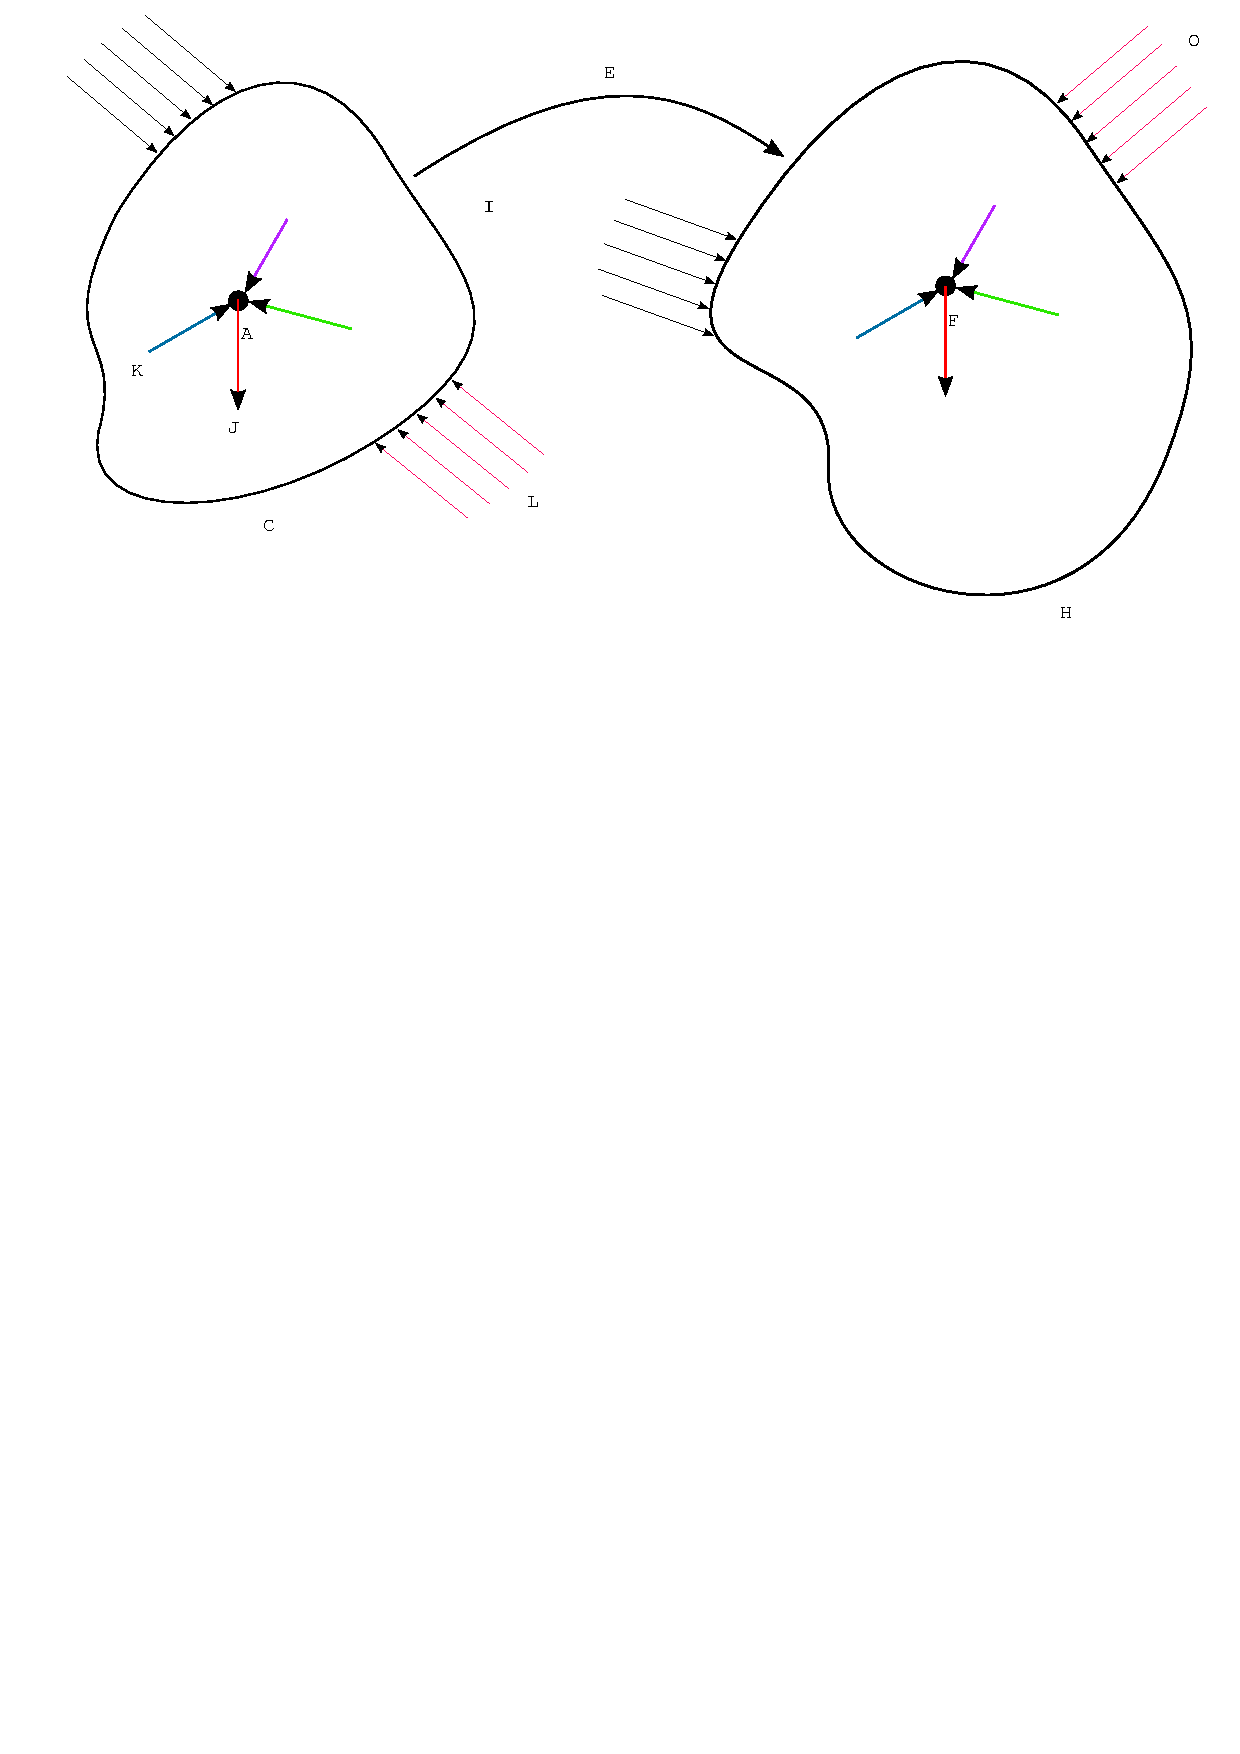
\includegraphics[width=0.8\textwidth]{images/elucidation/continuum-potato-momentum}
  \caption{Interaction forces, traction and body loads on the tissue.}
  \label{continuum-potato-momentum}
\end{figure}

In soft tissues, the species production rate and flux that appear on
the right hand-side in Equation~(\ref{localbalanceofmass}) are
strongly dependent on the local state of stress. To correctly model
this coupling, the balance of linear momentum should be solved to
determine the local state of strain and stress.

Recall that the deformation of the tissue is characterised by the map
$\Bvarphi(\bX,t)$. Recognising that, in tendons, the solid collagen
fibrils and fibroblasts do not undergo mass transport, the material
velocity of this species, $\bV = \partial\Bvarphi/\partial t$, is used
as the primitive variable for mechanics. Each remaining species can
undergo mass transport relative to the solid collagen. For this
purpose, it is useful to define the material velocity of a species
$\iota$ \emph{relative to the solid phase} as: $\bV^\iota =
(1/\rho_0^\iota)\bF\bM^\iota$. Thus, the total material velocity of a
species~$\iota$ is $\bV+\bV^\iota$.

The tissue is subjected to a surface traction, $\bT$, and a body force
per unit mass, $\bg$. We define the partial first Piola-Kirchhoff
stress tensor corresponding to species~$\iota$ as the portion of the
total stress borne by the species. Denoting this quantity by
$\bP^\iota$, the natural boundary condition then implies that $\bT =
\sum_{\iota}\bP^\iota\bN$ on $\partial\Omega_0$. Thus, $\bP^\iota\bN$
is the corresponding partial traction, as depicted in
Figure~\ref{continuum-potato-momentum}.

Recognising that the concentrations of solutes are low, and
consequently that they do not bear appreciable stress, the partial
stresses and momentum balance equation are defined only for the solid
collagen and fluid phases. Written in integral form, the balance of
momentum of species~$\iota$ over $\Omega_0$ is,

\begin{eqnarray}
\underbrace{\frac{\mathrm{d}}{\mathrm{d}t} \int\limits_{\Omega_0}
  \rho_0^\iota(\bV+\bV^\iota) \mathrm{d}V}_{\text{Rate of change of
    momentum}} &=& \underbrace{\int\limits_{\Omega_0} \rho^\iota_0\bg
  \mathrm{d}V + \int\limits_{\Omega_0} \rho^\iota_0\bq^\iota
  \mathrm{d}V}_{\text{Resultant body force}} +
\underbrace{\int\limits_{\Omega_0} \Pi^\iota(\bV+\bV^\iota)
  \mathrm{d}V}_{\text{Momentum being created}} \nonumber\\ & &+
\underbrace{\int\limits_{\partial \Omega_0}\bP^\iota\bN
  \mathrm{d}A}_{\text{Boundary traction}} -
\underbrace{\int\limits_{\partial
    \Omega_0}(\bV+\bV^\iota)\bM^\iota\cdot\bN
  \mathrm{d}A}_{\text{Momentum leaving the domain}},
\label{globalbalanceofmomentum}
\end{eqnarray}

\noindent where $\bq^\iota$ is the force per unit mass exerted upon
$\iota$ by the other species present. Note the contributions of the
mass source distributed through the volume and the influx over the
boundary to the rate of change of momentum in
Equation~(\ref{globalbalanceofmomentum}).

Writing $(\bV+\bV^\iota) \bM^\iota\cdot\bN$ as
$((\bV+\bV^\iota)\otimes\bM^\iota)\bN$, and using Gauss' divergence
theorem (Appendix~\ref{gauss-divergence}), one obtains:
\begin{eqnarray}
\int\limits_{\Omega_0} \left(\frac{\partial\rho_0^\iota}{\partial
  t}\left(\bV+\bV^\iota\right) + \rho_0^\iota\frac{\partial}{\partial
  t}\left(\bV+\bV^\iota\right)\right) \mathrm{d}V =
\int\limits_{\Omega_0}\rho^\iota_0\left(\bg+\bq^\iota\right)
\mathrm{d}V \qquad&
&\nonumber\\ +\int\limits_{\Omega_0}\left(\Pi^\iota\left(\bV+\bV^\iota\right)
+ \mathrm{DIV}[\bP^\iota]\right) \mathrm{d}V& & \nonumber\\ -
\int\limits_{\Omega_0}\mathrm{DIV}
\left[\left(\bV+\bV^\iota\right]\otimes\bM^\iota\right)\mathrm{d}V .
& &
\end{eqnarray}

\noindent Using the mass balance equation (\ref{localbalanceofmass}),
and applying Leibniz rule to the last term gives

\begin{eqnarray}
\int\limits_{\Omega_0} \rho_0^\iota\frac{\partial}{\partial
  t}\left(\bV+\bV^\iota\right) \mathrm{d}V &=&
\int\limits_{\Omega_0}\rho^\iota_0\left(\bg+\bq^\iota\right)
\mathrm{d}V \nonumber\\ & &+
\int\limits_{\Omega_0}\left(\mathrm{DIV}\left[\bP^\iota\right] -
\left(\mathrm{GRAD}\left[\bV+\bV^\iota\right]\right)\bM^\iota\right)
\mathrm{d}V, \nonumber
\end{eqnarray}

\noindent where $\mathrm{{GRAD}[\bullet]}$ is the gradient operator in
the reference configuration. Localising this result gives the balance
of linear momentum for a single species in $\Omega_{0}$:

\begin{equation}
\begin{split}
\rho_0^\iota\frac{\partial}{\partial t}\left(\bV+\bV^\iota\right) &
=\rho^\iota_0\left(\bg+\bq^\iota\right) +
\mathrm{DIV}[\bP^{\,\iota}]\\ & \quad -\left(\mathrm{GRAD}\left[\bV+
  \bV^\iota\right]\right)\bM^\iota, \quad \iota = \mathrm{c,f}
\label{localbalanceofmomentum}
\end{split}
\end{equation} 

The final term with the gradient of total species velocity identifies
the contribution of the flux to the balance of momentum. In practise,
when the relative magnitude of the fluid mobility (and hence flux) is
small, the final term on the right hand side of
Equation~(\ref{localbalanceofmomentum}) is negligible, resulting in a
more classical form of the balance of momentum. Furthermore, in the
absence of significant acceleration of the tissue during growth, the
left hand-side can also be neglected, reducing
(\ref{localbalanceofmomentum}) to the quasi-static balance of linear
momentum.

The interaction forces, $\bq^\iota$, satisfy a relation with the mass
sources, $\Pi^\iota$, that is elucidated by the following
argument. One way of arriving at the balance of momentum of the entire
tissue is by summing Equation~(\ref{globalbalanceofmomentum}) over
$\iota = \mathrm{c,f}$

\begin{eqnarray}
\sum\limits_{\iota}\frac{\mathrm{d}}{\mathrm{d}t}
\int\limits_{\Omega_0} \rho_0^\iota(\bV+\bV^\iota) \mathrm{d}V &=&
\sum\limits_{\iota}\int\limits_{\Omega_0} \rho^\iota_0\bg
\mathrm{d}V + \sum\limits_{\iota}\int\limits_{\Omega_0}
\rho^\iota_0\bq^\iota \mathrm{d}V\nonumber\\& & +
\sum\limits_{\iota}\int\limits_{\Omega_0} \Pi^\iota(\bV+\bV^\iota)
\mathrm{d}V + \sum\limits_{\iota} \int\limits_{\partial
\Omega_0}\bP^\iota\bN \mathrm{d}A\nonumber\\
& & - \sum\limits_{\iota}\int\limits_{\partial
\Omega_0}(\bV+\bV^\iota)\bM^\iota\cdot\bN \mathrm{d}A.
\label{momentumsummation}
\end{eqnarray}

As in Section~\ref{balance-of-mass}, recall that for an external
observer, the rate of change of momentum of the entire system is
affected by external agents only, and is independent of internal
interactions of any nature ($\bq^\iota$ and $\Pi^\iota$). This
observation leads to the following equivalent expression for the rate
of change of linear momentum of the system:

\begin{eqnarray}
\sum\limits_{\iota}\frac{\mathrm{d}}{\mathrm{d}t}
\int\limits_{\Omega_0} \rho_0^\iota(\bV+\bV^\iota) \mathrm{d}V &=&
\int\limits_{\Omega_0}\rho_0\bg \mathrm{d}V +
\int\limits_{\partial \Omega_0}\bP\bN \mathrm{d}A \nonumber\\
& &- \sum\limits_{\iota}\int\limits_{\partial
\Omega_0}(\bV+\bV^\iota)\bM^\iota\cdot\bN \mathrm{d}A.
\label{momentumexternal}
\end{eqnarray}

\noindent Here, $\bP = \sum\limits_{\iota}\bP^\iota$ and $\rho_0 =
\sum\limits_{\iota}\rho_0^\iota$. Since both (\ref{momentumsummation})
and (\ref{momentumexternal}) represent the balance of linear momentum
of the system, it follows upon inspection that:

\begin{eqnarray}
\sum\limits_{\iota}\int\limits_{\Omega_0} \rho^\iota_0\bq^\iota
\mathrm{d}V + \sum\limits_{\iota}\int\limits_{\Omega_0}
\Pi^\iota(\bV+\bV^\iota) \mathrm{d}V = 0.
\end{eqnarray}

\noindent Recalling the relation between the sources
(\ref{masssummationresult}), and localising leads to

\begin{eqnarray}
\sum\limits_{\iota}\left(\rho^\iota_0\bq^\iota +
\Pi^\iota\bV^\iota\right)=0,
\label{momentumsummationresult}
\end{eqnarray}

\noindent a result that is also consistent with classical mixture
theory \citep{TruesdellNoll:65}.

\subsection{Balance of angular momentum}
\label{balance-of-angular-momentum}

The balance of angular momentum in a purely mechanical theory implies
that the Cauchy stress is symmetric: $\Bsigma =
\Bsigma^{\mathrm{T}}$. This result is now examined in context of an
open system comprising of multiple interacting and inter-converting
species.

The balance of angular momentum about the origin, as observed from an
inertial reference frame, of a species~$\iota$ over $\Omega_{0}$
requires,

\begin{eqnarray}
\underbrace{\frac{\mathrm{d}}{\mathrm{d}t} \int\limits_{\Omega_0}
  \Bvarphi \times \rho^\iota_0(\bV+\bV^\iota)\mathrm{d}V}_{\text{Rate
    of change of angular momentum}} &=&
\underbrace{\int\limits_{\Omega_0}\Bvarphi\times\left
  [\rho^\iota_0\left(\bg+\bq^\iota\right) +
    \Pi^\iota\left(\bV+\bV^\iota\right)\right]\mathrm{d}V}_{\text{Moment
    from body forces and angular momentum being created}}
\nonumber\\ & &+ \underbrace{
  \int\limits_{\partial\Omega_0}\Bvarphi\times\left(\bP^\iota -
  \left(\bV+\bV^\iota\right)\otimes\bM^\iota\right)\bN
  \mathrm{d}A}_{\text{Moment from traction and angular momentum
    leaving the domain}}
\label{globalbalanceofangularmomentum}
\end{eqnarray}

\noindent Applying properties of the cross product, Gauss' divergence
theorem (Appendix~\ref{gauss-divergence}) and Leibniz rule gives

\begin{eqnarray}
\int\limits_{\Omega_0}\bV\times\rho^\iota_0\bV^\iota + \Bvarphi\times
\left(\frac{\partial\rho^\iota_0}{\partial
  t}\left(\bV+\bV^\iota\right)+ \rho^\iota_0\frac{\partial} {\partial
  t}\left(\bV+\bV^\iota\right)\right)\mathrm{d}V =\qquad\quad&
&\nonumber\\ \int\limits_{\Omega_0}\Bvarphi\times\rho^\iota_0
\left(\bg+\bq^\iota+\Pi^\iota\left(\bV+\bV^\iota\right)\right)
\mathrm{d}V& &\nonumber\\ +
\int\limits_{\Omega_0}\left(\Bvarphi\times\mathrm{DIV}[\bP^\iota] -
\Bvarphi\times\left(\mathrm{GRAD}
\left[\bV+\bV^\iota\right]\bM^\iota\right)\right)\mathrm{d}V &
&\nonumber\\ \int\limits_{\Omega_0}
\left(-\Bvarphi\times\left(\bV+\bV^\iota\right)
\mathrm{DIV}\left[\bM^\iota\right]\right) \mathrm{d}V & &\nonumber\\ -
\int\limits_{\Omega_0}\Bepsilon\colon\left(\left(\bP^\iota -
\left(\bV+\bV^\iota\right) \otimes\bM^\iota\right)
\bF^\mathrm{T}\right) \mathrm{d}V,\nonumber
\end{eqnarray}

\noindent where $\Bepsilon$ is the permutation symbol, and
$\Bepsilon\colon\bA$ is written as $\epsilon_{ijk}A_{jk}$ in
indicial form, for any second-order tensor $\bA$. Using the mass
balance equation (\ref{localbalanceofmass}), and balance of linear
momentum (\ref{localbalanceofmomentum}), we have
\begin{displaymath}
\int\limits_{\Omega_0}\bV\times\rho^\iota_0\bV^\iota\mathrm{d}V =
-\int\limits_{\Omega_0}\Bepsilon\colon
\left(\left(\bP^\iota-\left(\bV+\bV^\iota\right)
\otimes\underbrace{\bM^\iota}_{\rho_0^\iota\bF^{-1}\bV^\iota}\right)
\bF^\mathrm{T}\right)\mathrm{d}V. 
\end{displaymath}

\noindent Recalling the relation of the permutation symbol to the
cross product, and the indicated relation between $\bM^\iota$ and
$\bV^\iota$ leads to

\begin{equation}
\bzero =
-\int\limits_{\Omega_0}\Bepsilon\colon\left(\left(\bP^\iota-\bV^\iota
\otimes \rho_0^\iota\bF^{-1}\bV^\iota\right)
\bF^\mathrm{T}\right)\mathrm{d}V.\nonumber
\end{equation}

\noindent Localising this result and again applying the properties of
the permutation symbol leads to the symmetry condition,

\begin{equation}
\left(\bP^\iota-\bV^\iota\otimes\rho^\iota_0\bF^{-1}\bV^\iota\right)
\bF^\mathrm{T} = \bF\left(\bP^\iota-\bV^\iota \otimes
\rho^\iota_0\bF^{-1}\bV^\iota\right)^\mathrm{T}.
\label{localbalanceofangularmomentum}
\end{equation}

\noindent But, $(\bV^\iota\otimes\bF^{-1}\bV^\iota)\bF^\mathrm{T} =
\bV^\iota\otimes\bV^\iota$, and thus, the symmetry
$\bP^\iota\bF^\mathrm{T} = \bF(\bP^\iota)^\mathrm{T}$ that results
from conservation of angular momentum for a purely mechanical theory
is retained in this case of a mixture. The partial Cauchy stresses are
therefore symmetric: $\Bsigma^\iota = \Bsigma^{\iota^\mathrm{T}}$, and
this is also seen directly in terms of spatial quantities in
Section~\ref{eu-balance-of-angular-momentum}.

Divergent results on this topic (in terms of which stress-like
quantities are deduced symmetric) stem primarily from the exact
definitions of the fundamental quantities involved in the
analysis. This is especially true of how the total stress in the
system is distributed as partial stresses borne by the species
comprising the system. For e.g., \citet{EpsteinMaugin:2000}
incorporate an ``irreversible'' contribution from their species flux
into their local measure of partial Cauchy stress. This results in
their deduction of a non-symmetric partial Cauchy stress, in contrast
to the result shown above.

\subsection{Balance of energy}
\label{balance-of-energy}

\begin{figure}[ht]
  \centering
  \psfrag{A}{$\bX$}
  \psfrag{B}{\renewcommand{\baselinestretch}{1.5}$r^\iota$}
  \psfrag{E}{$\Bvarphi$}
  \psfrag{C}{$\Omega_0$}
  \psfrag{L}{$\bP\bN$}
  \psfrag{K}{$\tilde{e}^\iota$}
  \psfrag{D}{$\bN\cdot\bQ$}
  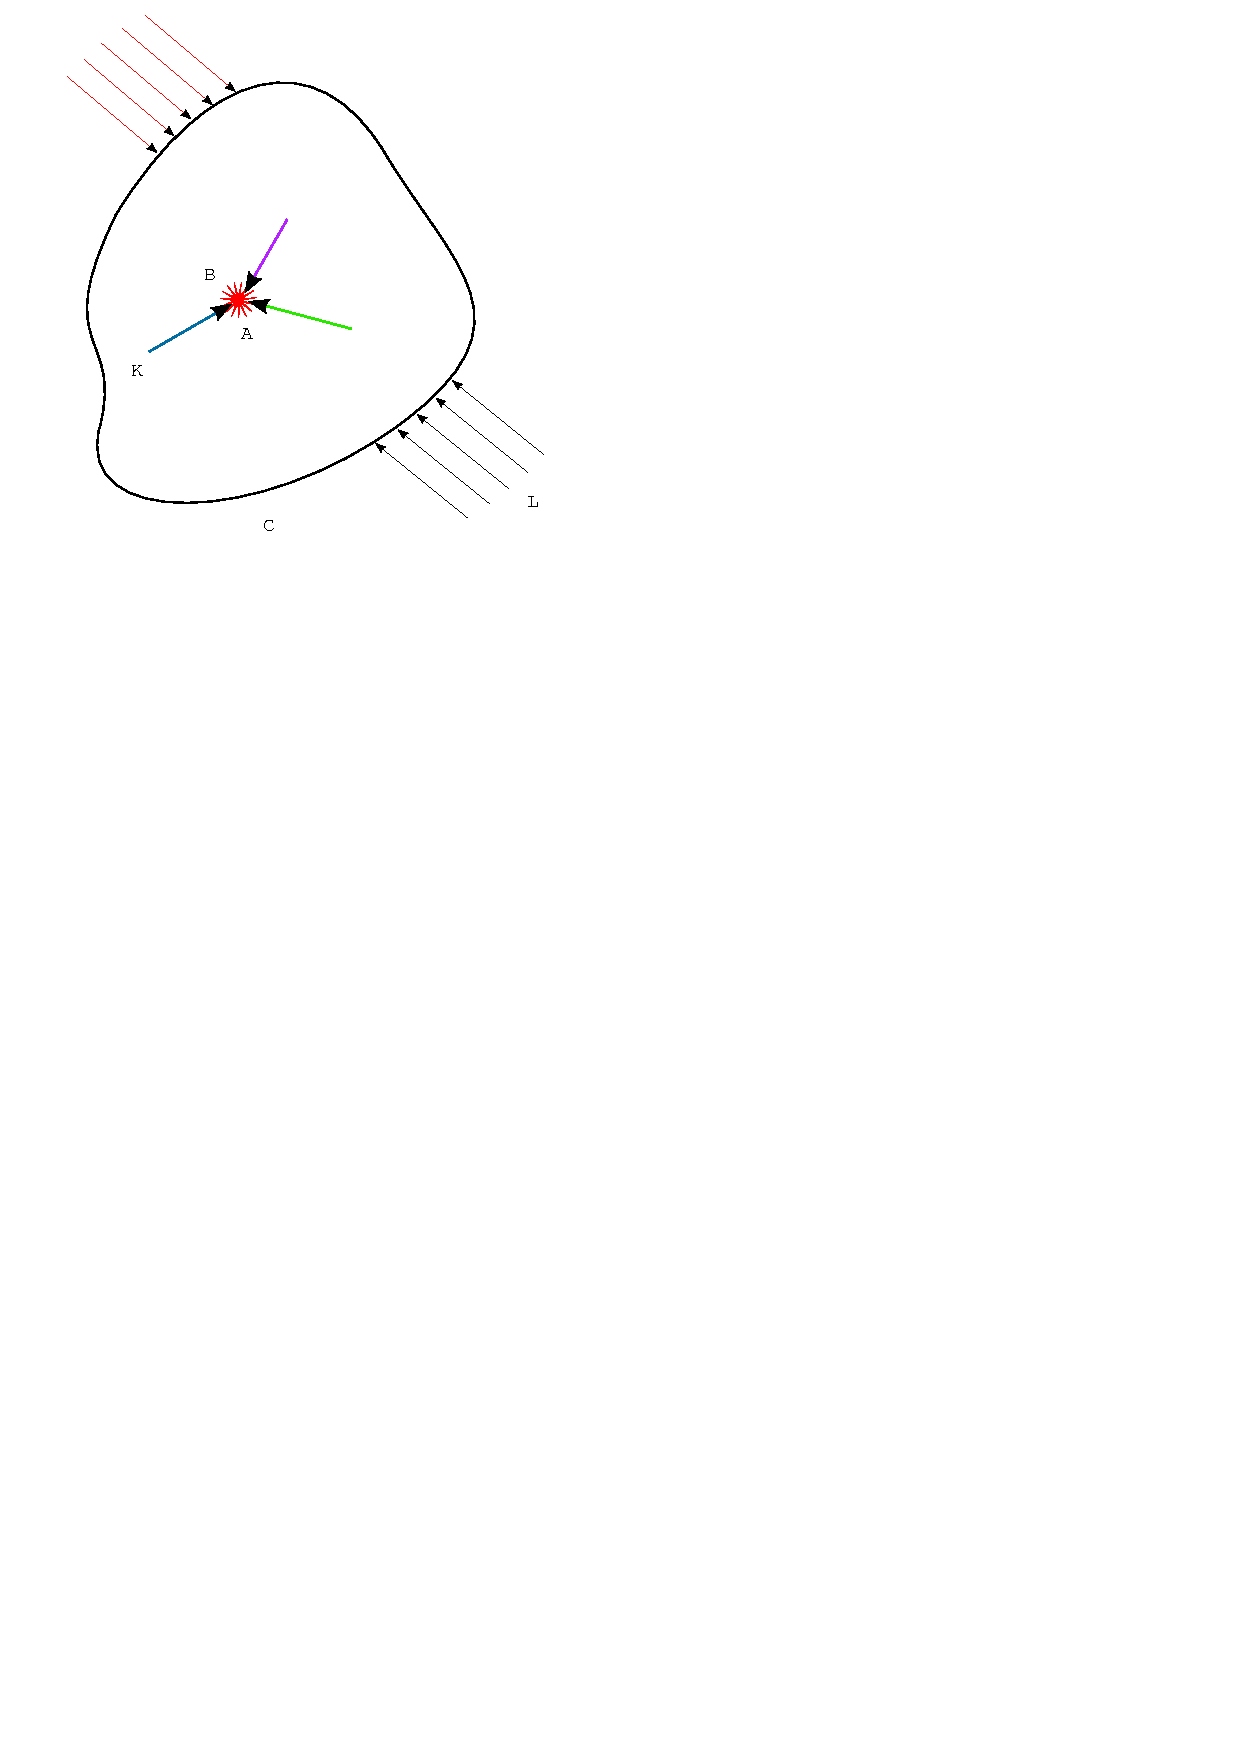
\includegraphics[width=0.4\textwidth]{images/elucidation/continuum-potato-energy}
  \caption{Energetic interactions the tissue is subjected to.}
  \label{continuum-potato-energy}
\end{figure}

Since the masses of the various species constituting the system are
allowed to change as a result of mass transport and interconversion,
it is appropriate to work with energy and energy-like quantities per
unit mass. In addition to the terms introduced previously, the
internal energy per unit mass of species~$\iota$ is denoted $e^\iota$;
the heat supply to species~$\iota$ per unit mass of that species is
$r^\iota$; and the partial heat flux vector of $\iota$ is $\bQ^\iota$,
defined on $\Omega_0$. An interaction energy appears between species:
The energy transferred to $\iota$ by all other species is
$\tilde{e}^\iota$, per unit mass of $\iota$. These quantities are
shown in Figure~\ref{continuum-potato-energy}.

Working in $\Omega_0$, the rate of change of internal and kinetic
energies of species~$\iota$ is related to the work done on it by
mechanical loads, processes of mass production and transport, heating
and energy transfer as:

\begin{eqnarray}
\underbrace{\frac{\mathrm{d}}{\mathrm{d}t}
  \int\limits_{\Omega_0}\rho_0^\iota 
\left ( e^\iota + \frac{1}{2} \Vert\bV+\bV^\iota\Vert^2 \right )
\mathrm{d}V}_{\text{Rate of change of energy}} =
\underbrace{\int\limits_{\Omega_0} \left(\rho_0^\iota\bg 
\cdot\left(\bV+\bV^\iota\right) + \rho_0^\iota r^\iota
\right)\mathrm{d}V}_{\text{Work done by body forces and heat
    supplied}}\qquad& &\nonumber\\ 
+\underbrace{\int\limits_{\Omega_0} \rho_0^\iota\bq^\iota\cdot(\bV +
  \bV^\iota) \mathrm{d}V}_{\text{Work done by interaction forces}}&
&\nonumber\\ 
+ \underbrace{\int\limits_{\Omega_0} \left(\Pi^\iota\left(e^\iota +
\frac{1}{2}\Vert\bV+\bV^\iota\Vert^2\right) +
\rho^\iota_0\tilde{e}^\iota\right)\mathrm{d}V}_{\text{Energy being created}} 
& & \nonumber \\ 
+ \underbrace{\int\limits_{\partial \Omega_0}
  \left(\left(\bV+\bV^\iota\right)\cdot\bP^\iota - 
\bM^\iota\left(e^\iota +\frac{1}{2}
\Vert\bV+\bV^\iota\Vert^2\right) -
\bQ^\iota\right)\cdot\bN\mathrm{d}A}_{\text{Work done by applied
    traction and energy leaving the domain as mass and heat flux}}.
\label{globalbalanceofenergy}
\end{eqnarray}

The above equation for the rate of change of energy of a single
species can be further simplified by applying Gauss' divergence
theorem (Appendix~\ref{gauss-divergence}) and Leibniz rule, giving
first,

\begin{eqnarray}
\int\limits_{\Omega_0}\left(\frac{\partial\rho_0^\iota}{\partial t}
\left(e^\iota + \frac{1}{2}\Vert\bV+\bV^\iota\Vert^2 \right) +
\rho^\iota_0\frac{\partial}{\partial t}\left(e^\iota +
\frac{1}{2}\Vert\bV+\bV^\iota\Vert^2 \right)\right) \mathrm{d}V
=\qquad & &\nonumber\\ \int\limits_{\Omega_0} \left(\rho_0^\iota\bg
\cdot\left(\bV+\bV^\iota\right) + \rho_0^\iota r^\iota +
\Pi^\iota\left(e^\iota +
\frac{1}{2}\Vert\bV+\bV^\iota\Vert^2\right) +
\rho^\iota_0\tilde{e}^\iota\right)\mathrm{d}V& 
& \nonumber
\\ +\int\limits_{\Omega_0}\rho_0^\iota\bq^\iota\cdot(\bV+\bV^\iota)
\mathrm{d}V&
&\nonumber\\ +\int\limits_{\Omega_0} \left(\left(\bV+\bV^\iota\right)
\cdot\mathrm{DIV}\left[\bP^\iota\right]
+ \bP^\iota\colon\mathrm{GRAD}
\left[\bV+\bV^\iota\right]\right) \mathrm{d}V& &\nonumber\\ -
\int\limits_{\Omega_0}\left(\mathrm{DIV}\left[\bM^\iota\right]
\left(e^\iota +\frac{1}{2}
\Vert\bV+\bV^\iota\Vert^2\right)\right)\mathrm{d}V & 
&\nonumber\\ -\int\limits_{\Omega_0}\left(
\left(\mathrm{GRAD}\left[e^\iota\right]+
\left(\bV+\bV^\iota\right) \cdot
\mathrm{GRAD}\left[\bV+\bV^\iota\right]\right) \cdot\left(\bM^\iota\right)
- \mathrm{DIV}\left[\bQ^\iota\right]\right)\mathrm{d}V.\nonumber
\end{eqnarray}

\noindent Applying the balance of mass (\ref{localbalanceofmass}) and
the balance of momentum (\ref{localbalanceofmomentum}) to the equation
above and localising the result, we have,

\begin{eqnarray}
\rho^\iota_0\frac{\partial e^\iota}{\partial t} &=&
\bP^\iota\colon\mathrm{GRAD}\left[\bV+\bV^\iota\right]-
\mathrm{DIV}\left[\bQ^\iota\right] + \rho_0^\iota r^\iota
+\rho^\iota_0\tilde{e}^\iota\nonumber\\
& & - \mathrm{GRAD}\left[e^\iota\right]\cdot\bM^\iota,
\label{localbalanceofenergy}
\end{eqnarray}

\noindent a final form of the balance of energy of a species~$\iota$
which is most convenient for combining with the entropy inequality,
leading to the Clausius-Duhem form of the dissipation inequality
(Section~\ref{entropy-inequality}).

Analogous to the results obtained in Sections~\ref{balance-of-mass}
and \ref{balance-of-linear-momentum} the inter-species energy
transfers, $\tilde{e}^{\iota}$, are related to interaction forces,
$\bq^{\iota}$, and mass sources, $\Pi^{\iota}$. To demonstrate this,
we first obtain the balance of mass of the entire system by summing
Equation~\ref{globalbalanceofenergy} over all species:

\begin{eqnarray}
\sum\limits_{\iota}\frac{\mathrm{d}}{\mathrm{d}t}
\int\limits_{\Omega_0}\rho_0^\iota \left ( e^\iota + \frac{1}{2}
\Vert\bV+\bV^\iota\Vert^2 \right ) \mathrm{d}V =
\sum\limits_{\iota}\int\limits_{\Omega_0} \left(\rho_0^\iota\bg
\cdot\left(\bV+\bV^\iota\right) + \rho_0^\iota r^\iota
\right)\mathrm{d}V& &\nonumber\\ +
\sum\limits_{\iota}\int\limits_{\Omega_0}
\rho_0^\iota\bq^\iota\cdot(\bV+\bV^\iota)\mathrm{d}V& &\nonumber\\ +
\sum\limits_{\iota}\int\limits_{\Omega_0} \left(\Pi^\iota\left(e^\iota
+ \frac{1}{2}\Vert\bV+\bV^\iota\Vert^2\right) +
\rho^\iota_0\tilde{e}^\iota\right)\mathrm{d}V \label{energysummation}&
& \\ +\sum\limits_{\iota}\int\limits_{\partial
  \Omega_0}\left(\left(\bV+\bV^\iota\right)\cdot\bP^\iota -
\bM^\iota\left(e^\iota +\frac{1}{2} \Vert\bV+\bV^\iota\Vert^2\right) -
\bQ^\iota\right)\cdot\bN\mathrm{d}A.\quad& & \nonumber
\end{eqnarray}

Expressing the rate of change of energy of the system interacting with
its environment from the point of view of an external observer unaware
of internal interactions between species (interaction forces, mass
interconversion and inter-species energy transfers), we have,

\begin{eqnarray}
\sum\limits_{\iota}\frac{\mathrm{d}}{\mathrm{d}t}
\int\limits_{\Omega_0}\rho_0^\iota \left ( e^\iota + \frac{1}{2}
\Vert\bV+\bV^\iota\Vert^2 \right ) \mathrm{d}V =
\sum\limits_{\iota}\int\limits_{\Omega_0} \left(\rho_0^\iota\bg
\cdot\left(\bV+\bV^\iota\right) + \rho_0^\iota r^\iota
\right)\mathrm{d}V &
&\nonumber\\ +\sum\limits_{\iota}\int\limits_{\partial
  \Omega_0}\left(\left(\bV+\bV^\iota\right)\cdot\bP^\iota -
\bM^\iota\left(e^\iota +\frac{1}{2} \Vert\bV+\bV^\iota\Vert^2\right) -
\bQ^\iota\right)\cdot\bN\mathrm{d}A.\quad\nonumber& &
\end{eqnarray}

Since the equation above and (\ref{energysummation}) are equivalent
statements of the balance of energy, it follows upon localisation
that,

\begin{eqnarray}
\sum\limits_{\iota}\left(\rho_0^\iota\bq^\iota\cdot(\bV+\bV^\iota)
+ \Pi^\iota\left(e^\iota +
\frac{1}{2}\Vert\bV+\bV^\iota\Vert^2\right) +
\rho^\iota_0\tilde{e}^\iota\right) =
0. \label{energysummationresult}
\end{eqnarray}

This result relating the interaction energies to interaction
forces between species, their sources and relative velocities, is
identical to that obtained from classical mixture theory
\citep{TruesdellNoll:65}, ensuring consistency of the present
formulation with mixture theory.

\section{The kinematics of growth}
\label{kinematics-of-growth}

\begin{figure}[ht]
  \centering
  \psfrag{A}{$\Omega_0$}
  \psfrag{B}{$\Omega^\ast$}
  \psfrag{C}{$\Omega_t$}
  \psfrag{D}{$\bX$}
  \psfrag{E}{$\bX^\ast$}
  \psfrag{F}{$\bx$}
  \psfrag{G}{$\bF^{\mathrm{g}^{\mathrm{\iota}}}$}
  \psfrag{H}{$\widetilde{\bF}^{\mathrm{e}^{\mathrm{\iota}}}$}
  \psfrag{I}{$\widetilde{\bF}$}
  \psfrag{J}{$\overline{\bF}^\mathrm{e}$}
  \psfrag{K}{$\bF$}
  \psfrag{L}{$\Bkappa$}
  \psfrag{M}{$\bu^\ast$}
  \psfrag{N}{$\Bvarphi$}
  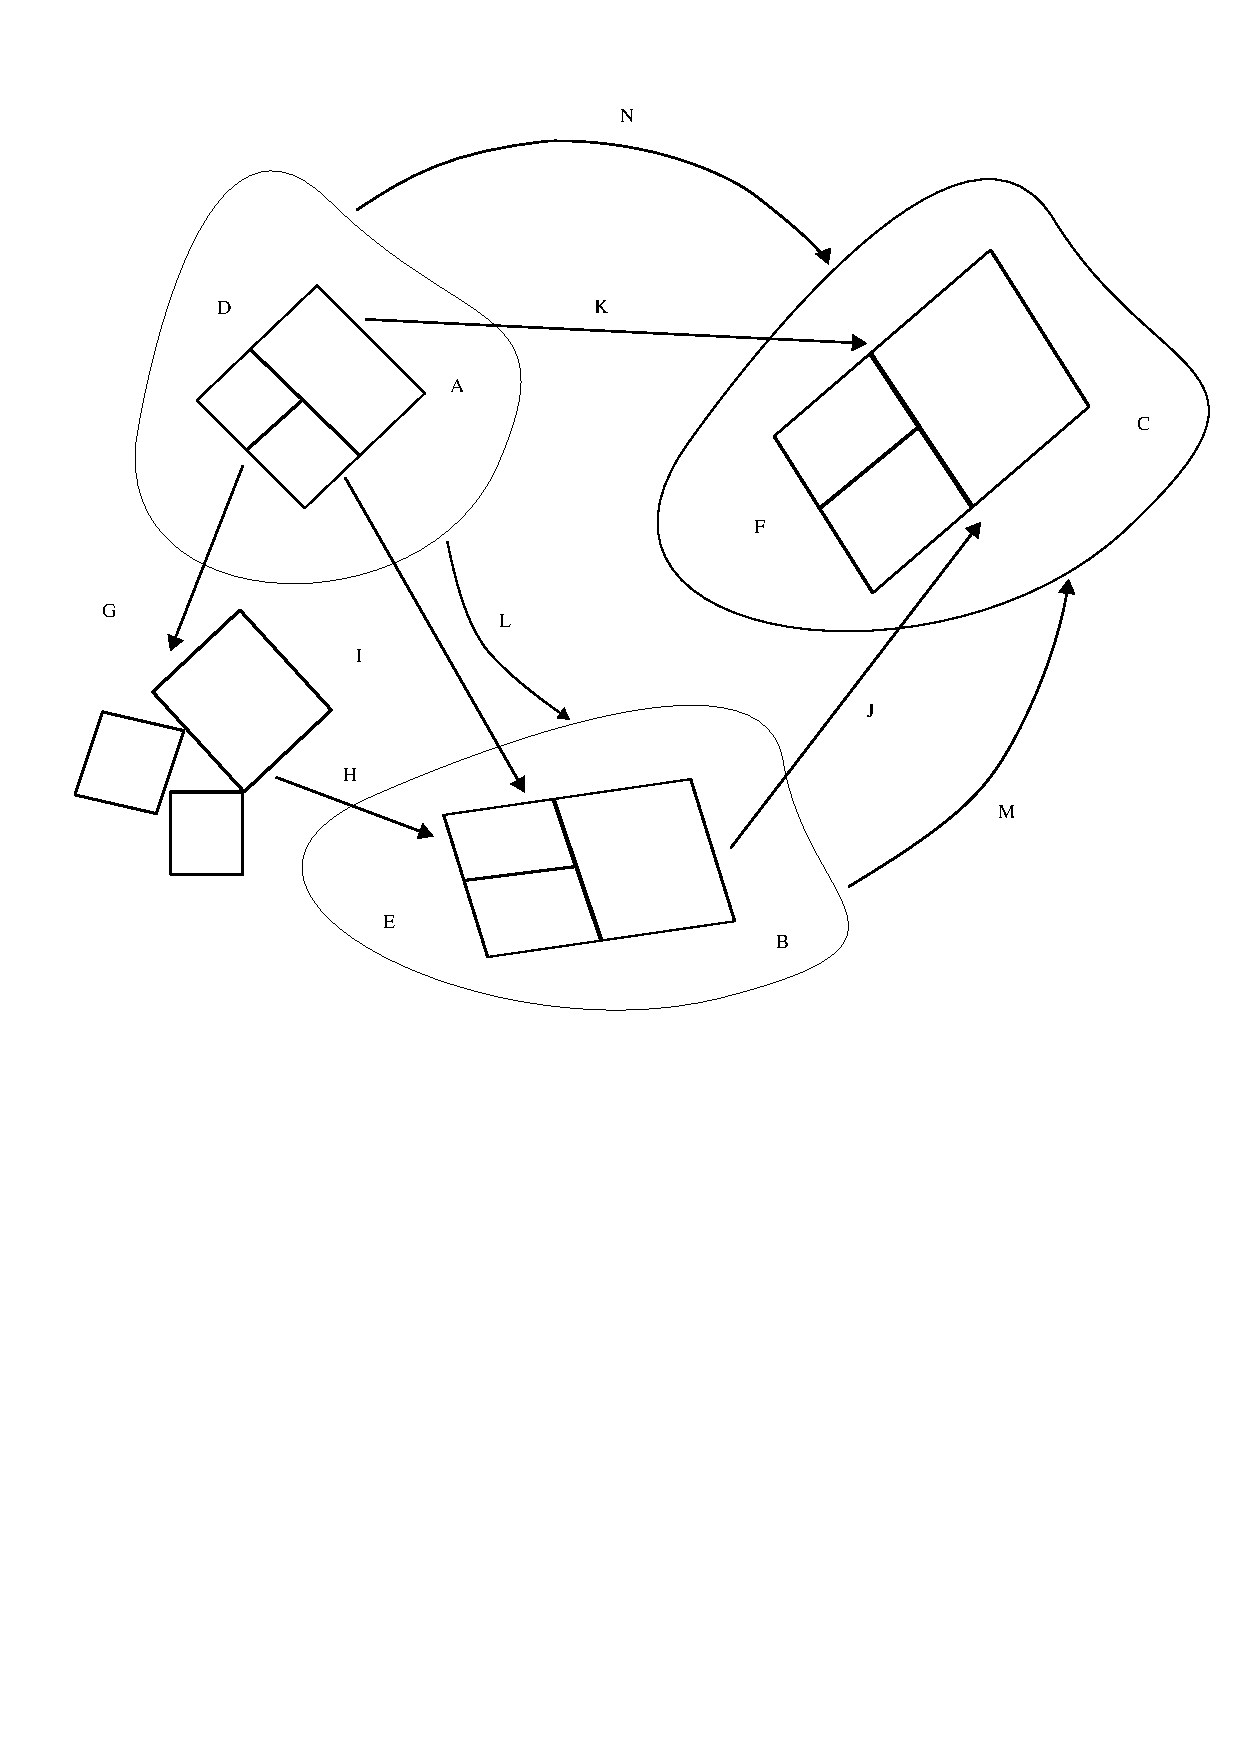
\includegraphics[width=0.8\textwidth]{images/elucidation/kinematics}
  \caption{The kinematics of growth, which holds for $\iota =
    \mathrm{c,f}$.} 
  \label{continuum-potato-growth-kinematics}
\end{figure}

Local volumetric changes are associated with changes in the
concentrations of solid collagen and fluid, $\iota = \mathrm{c,f}$,
and one important aspect of the coupling between mass transport and
mechanics stems from this phenomenon.\footnote{Another important facet
  of this coupling arises from the thermodynamically-motivated
  constitutive relationship for fluid flux, as detailed in
  Section~\ref{fluid-flux-constitutive-relationships}} If the material
of the solid collagen or fluid remains stress free, it swells with an
increase in concentration (mass of the species per unit system
volume), and shrinks as its concentration decreases. This leads to the
notion of a \emph{growth deformation gradient}.  This observation has
led to an active field of study within the literature on biological
growth \citep{Skalak:81, SkalakHoger:96, Klischetal:2001,
  TaberHumphrey:2001, LubardaHoger:02, AmbrosiMollica:2002}, and the
treatment below follows in the same vein.

In the setting of finite strain kinematics, the total deformation
gradient, $\bF$, is decomposed into the growth component of the solid
collagen, $\bF^{\mathrm{g}^\mathrm{c}}$, a
\emph{geometrically-necessitated elastic component} accompanying
growth, $\widetilde{\bF}^{\mathrm{e}^\mathrm{c}}$ and an
\emph{additional elastic component due to external stress},
$\overline{\bF}^{\mathrm{e}^\mathrm{c}}$. Later, we will write
$\bF^{\mathrm{e}^\mathrm{c}} = \overline{\bF}^{\mathrm{e}^\mathrm{c}}
\widetilde{\bF}^{\mathrm{e}^\mathrm{c}}$. This elastic-growth
decomposition is visualised in
Figure~\ref{continuum-potato-growth-kinematics} and is elaborated upon
below.

This split of the total deformation gradient is analogous to the
classical decomposition of multiplicative plasticity
\citep{Bilbyetal:1956,Lee:1969}. As explained in Section
\ref{role-of-current-mass-balance}, we assume that the fluid-filled
pores also deform with $\bF$, and that a component,
$\bF^{\mathrm{e}^\mathrm{f}}$, of this total deformation gradient
tensor, determines the fluid stress. We also assume a fluid growth
component, $\bF^{\mathrm{g}^\mathrm{f}}$, which is detailed below, and
that $\bF^{\mathrm{e}^\mathrm{f}}\bF^{\mathrm{g}^\mathrm{f}} =
\bF$. As with the solid collagen we admit $\bF^{\mathrm{e}^\mathrm{f}}
= \overline{\bF}^{\mathrm{e}^\mathrm{f}}
\widetilde{\bF}^{\mathrm{e}^\mathrm{f}}$, the sub-components carrying
the same interpretation as for the solid collagen. However, this last
decomposition is not explicitly used.

Assuming that the volume changes associated with growth described
above are isotropic, a simple form for the growth part of the
deformation gradient tensor is

\begin{equation}
\bF^{\mathrm{g}^\iota} = \left(
  \frac{\rho_0^\iota}{\rho_{0_{\mathrm{ini}}}^\iota} \right)^
  {\frac{1}{3}} 
{\bf 1},\quad \iota = \mathrm{c,f}
\label{isotropicgrowth} 
\end{equation} 

\noindent where $\rho_{0_{\mathrm{ini}}}^\iota(\bX)$ is the reference
concentration at the initial time, and {\bf 1} is the second-order
isotropic tensor.\footnote{This choice is only the simplest
  possible. Given the highly directional micro-structure and
  mechanical properties of many tissues, it seems likely that
  anisotropic growth (e.g., Wolff's law) is actually more common, as
  suggested by the thermodynamic arguments presented in
  Section~\ref{eu-stress-dependent-source}.} In the state $\bF =
\bF^{\mathrm{g}^\iota}$, the species would be stress free. The
kinematics being local, the action of $\bF^{\mathrm{g}^\iota}$ alone
can result in incompatibility, which is eliminated by the
geometrically-necessary elastic deformation
$\widetilde{\bF}^{\mathrm{e}^{\mathrm{\iota}}}$, which causes an
internal, self-equilibrated stress. The component
$\overline{\bF}^{\mathrm{e}^\iota}$ is associated with a a separate
elastic deformation due to an external stress.

\subsection{Saturation and tissue swelling}
\label{saturation-and-tissue-swelling}

\begin{figure}[ht]
  \begin{center}
    \psfrag{A}{\small A}
    \psfrag{B}{\small B}
    \psfrag{C}{\small B}
    \psfrag{D}{\small C}
    \psfrag{E}{\small Unsaturated}
    \psfrag{F}{\small Saturated}
    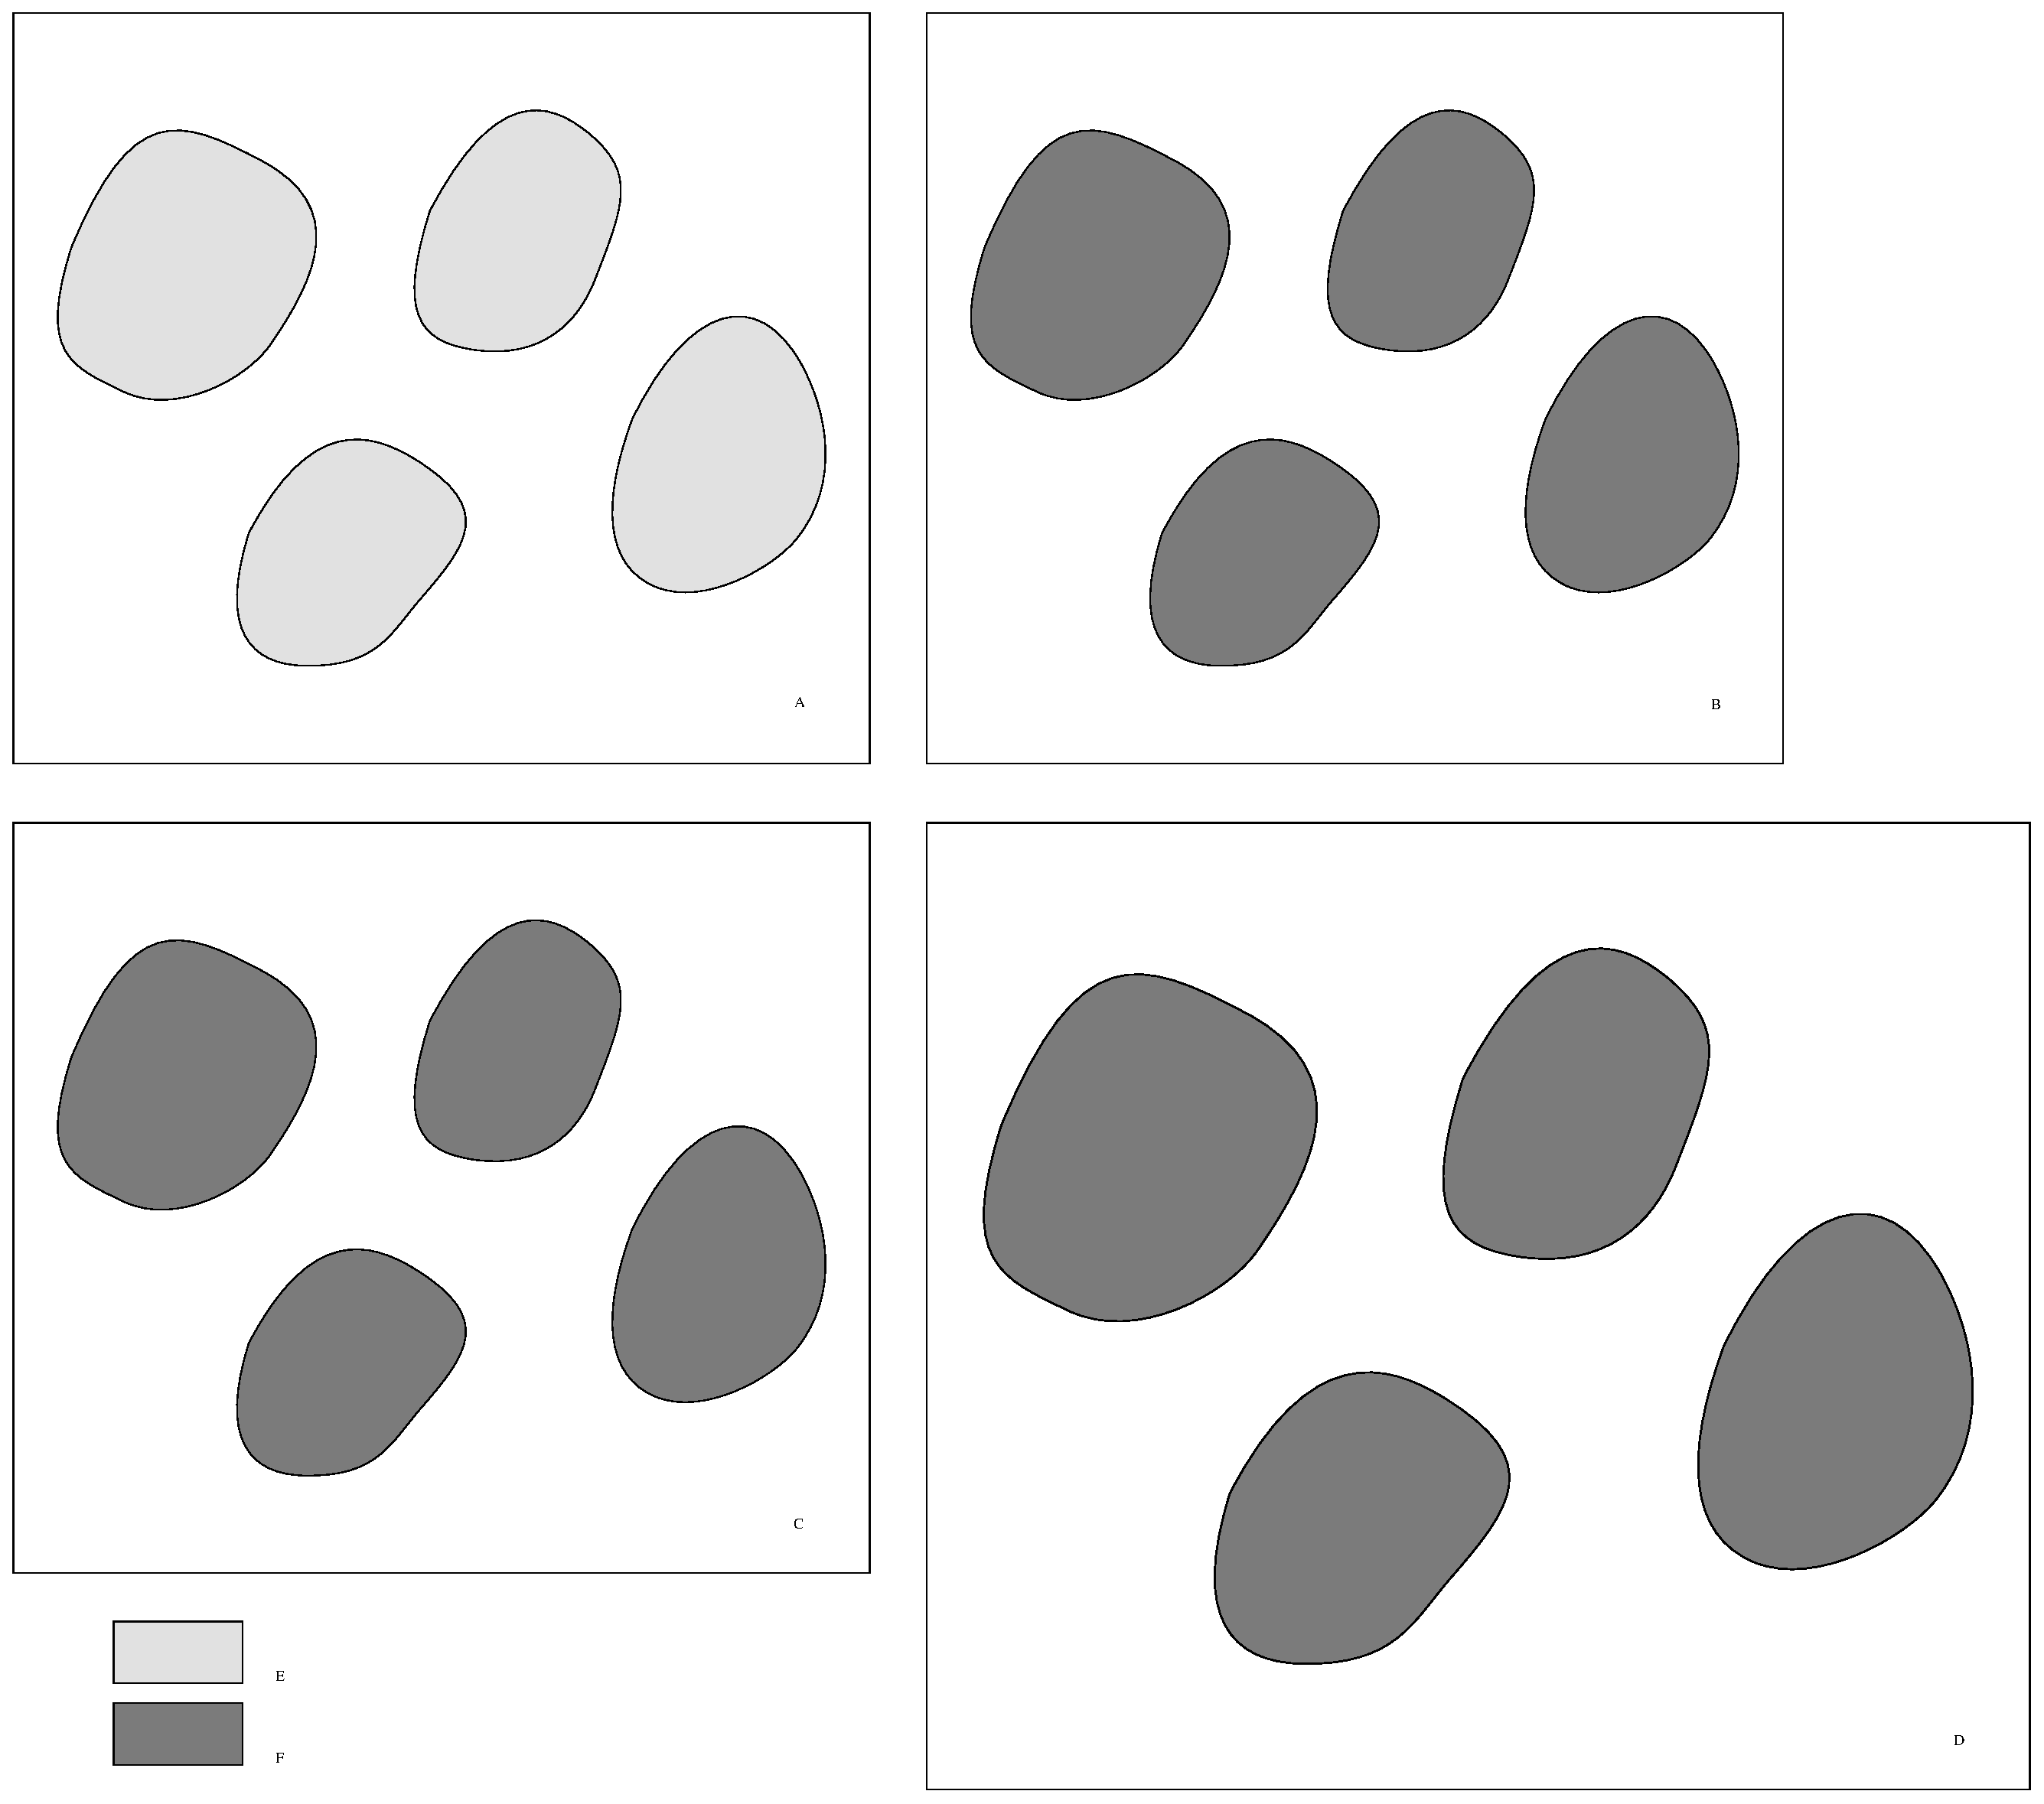
\includegraphics[width=0.8\textwidth]{images/elucidation/saturation-stages}
    \caption{Stages of tissue saturation.}
  \end{center}
      {Unsaturated tissue in the current configuration (A) allows
        influx of fluid without swelling until it is completely
        saturated (B). Initially saturated tissue (B), in general,
        swells with influx of fluid (C).}
      \label{saturation-and-swelling}
\end{figure}

\noindent The degree of saturation of the solid phase plays a
fundamental role in determining whether the tissue responds to an
infusion (expulsion) of fluid by swelling (shrinking). In particular,
the isotropic swelling law defined by Equation (\ref{isotropicgrowth})
has to be generalised to treat the case in which the solid phase is
not saturated by fluid.

Figure~\ref{saturation-and-swelling} schematically depicts two
possible scenarios. If the tissue is unsaturated in its current
configuration, as in A, then, on a microscopic scale, it contains
unfilled voids. It is thus capable of allowing an influx of fluid,
which tends to increase its degree of saturation until fully
saturated, as in B. This increase does not cause swelling of the
tissue in the local stress-free state, as there is free volume for
incoming fluid to occupy. However, once the tissue is saturated in the
current configuration, an increase in the fluid content causes
swelling in the stress-free state, as depicted in C, since there is no
free volume for the entering fluid to occupy. It is this second case
that is modelled by (\ref{isotropicgrowth}).

It is worth emphasising that this argument holds for
$\bF^{\mathrm{g}^\mathrm{f}}$, which is the local stress-free state of
deformation of the fluid-containing pores at a point. The actual
deformation gradient, $\bF =
\bF^{\mathrm{e}^\mathrm{f}}\bF^{\mathrm{g}^\mathrm{f}}$, also depends
on the the elastic part, $\bF^{\mathrm{e}^\mathrm{f}}$, which is
determined by the constitutive response of the fluid. Under stress, an
incompressible fluid will have
$\mathrm{det}\bF^{\mathrm{e}^\mathrm{f}} = 1$, where
$\mathrm{det}\cdot$ denotes the determinant of a second-order
tensor. Therefore a fluid-saturated tissue will swell with fluid
influx, $\mathrm{det}\bF = \mathrm{det}\bF^{\mathrm{g}^\mathrm{f}} >
1$. A compressible fluid may have
$\mathrm{det}\bF^{\mathrm{e}^\mathrm{f}} < 1$ allowing
$\mathrm{det}\bF < 1$ even with
$\mathrm{det}\bF^{\mathrm{g}^\mathrm{f}} >1$. Even in this case,
however, in the stress-free state there will be swelling.

Therefore, for the fluid phase, the isotropic swelling law can be
extended to the unsaturated case by introducing a degree of
saturation, $\tilde{v}^\iota$, defined in the current configuration,
$\Omega_t$. We have $\tilde{v}^\iota = \rho^\iota/\tilde{\rho}^\iota$,
where $\tilde{\rho}^\iota$ is the intrinsic density in $\Omega_t$ and
is given by $\tilde{\rho}^\iota =
\tilde{\rho}^\iota_0/\mathrm{det}\bF$. Note that the intrinsic
reference density, $\tilde{\rho}^\iota_0$, is a material
property. Upon solution of the mass balance equation
(\ref{current-mass-balance}) for $\rho^\iota$, the species volume fractions,
$\tilde{v}^\iota$, can therefore be computed in a straightforward
fashion. The sum of these volume fractions is our required measure of
saturation defined in $\Omega_t$. Also, recognising that for the
dilute solutions obtained with physiologically-relevant solute
concentrations, the saturation condition is very well approximated by
$\tilde{v}^\mathrm{f} + \tilde{v}^\mathrm{c} = 1$, we proceed to
redefine the fluid growth-induced component of the pore deformation
gradient tensor as follows:

\begin{equation}
\bF^{\mathrm{g}^\mathrm{f}} = \left\{ \begin{array}{ll} \left(
  \frac{\rho_0^\mathrm{f}}{\rho_{0_{\mathrm{sat}}}^\mathrm{f}}
  \right)^ {\frac{1}{3}}{\bf 1},& \tilde{v}^\mathrm{f} +
  \tilde{v}^\mathrm{c} = 1 \\ {\bf 1},& \mathrm{otherwise.}
\end{array}\right.
\label{saturation}
\end{equation}

\noindent In Equation~(\ref{saturation}), $\rho_{0_{\mathrm{sat}}}^\mathrm{f}$
is the reference concentration value at which the tissue attains
saturation in the current configuration.

With this redefinition of $\bF^{\mathrm{g}^\mathrm{f}}$, it is
implicit that $\tilde{v}^\mathrm{f} + \tilde{v}^\mathrm{c} > 1$ is
non-physical. Saturation holds in the sense that $\tilde{v}^\mathrm{f}
+ \tilde{v}^\mathrm{c} = 1$. It has been common in soft tissue
literature to assume that, under normal physiological conditions, soft
tissues are fully saturated by the fluid and
\mbox{Equation~(\ref{isotropicgrowth})} is appropriate for $\iota =
\mathrm{f}$. However, this treatment of saturation and swelling
induced by the fluid phase is necessary background for Section
\ref{caviation-under-tension}, where we examine the response of the
fluid phase under tension. This approach also holds relevance for
partial drying, which \emph{ex vivo} or \emph{in vitro} tissue may be
subject to under certain laboratory conditions. It also significantly
expands the relevance of formulation by making it applicable to the
mechanics of drained porous media other than biological tissue, most
prominently, soils.

\section{The entropy inequality and its restrictions on constitutive
  relations}
\label{entropy-inequality}

The treatment presented in this section builds upon certain
fundamental assumptions underlying the system under
consideration. Firstly, the Second Law of thermodynamics (or the
entropy production inequality) is assumed to hold at a continuum point
for all species as a whole, but, in general, not for each individual
species. Differing views on the spatial scale at which a continuum
point is defined lead to varying interpretations of the Second
Law. The spatial scale of our continuum point is chosen such that the
following arguments are valid. Another assumption that is tied to this
spatial scale, and consequently to the degree of observed homogeneity
between mixed species, is that all species occupying a continuum point
in the tissue have the same absolute temperature, $\theta$.

With these assumptions, and denoting by $\eta^\iota$ the entropy per
unit mass of species~$\iota$, the entropy inequality, when written out
for the entire system in the reference configuration, reads

\begin{eqnarray}
\underbrace{\sum\limits_{\iota}\frac{\mathrm{d}}{\mathrm{d}t}
  \int\limits_{\Omega_0} \rho_0^\iota \eta^\iota
  \mathrm{d}V}_{\text{Rate of change of entropy}} &\geq&
\underbrace{\sum\limits_{\iota}\int\limits_{\Omega_0}\left( \Pi^\iota
  \eta^\iota + \frac{\rho_0^\iota r^\iota}{\theta}\right)
  \mathrm{d}V}_{\text{Entropy added through mass creation and heat
    supply}}\nonumber\\ & &- \underbrace{\sum\limits_{\iota}\int\limits_{\partial
  \Omega_0} \left(\bM^\iota \cdot \bN\eta^\iota +
\frac{\bQ^\iota}{\theta} \cdot \bN \right)\mathrm{d}A}_{\text{Entropy
      lost through mass and heat flux}}.
\label{globalentropyinequality}
\end{eqnarray}

\noindent Applying Gauss' divergence theorem
(Appendix~\ref{gauss-divergence}), using the mass balance equation
(\ref{localbalanceofmass}), and localising the result, we have the
following form of the entropy inequality,

\begin{equation}
\sum\limits_{\iota}\rho_0^\iota\frac{\partial\eta^\iota}{\partial
t} \geq \sum\limits_{\iota}\left(\frac{\rho_0^\iota
r^\iota}{\theta} -\mathrm{GRAD}\left[\eta^\iota\right]\cdot\bM^\iota -
\frac{\mathrm{DIV}\left[\bQ^\iota\right]}{\theta} +
\frac{\mathrm{GRAD}\left[\theta\right]\cdot\bQ^\iota}{\theta^2}\right).
\label{localentropyinequality}
\end{equation}

Now, multiplying Equation~(\ref{localentropyinequality}) by the
temperature field, $\theta$, subtracting it from the balance of
energy~(\ref{localbalanceofenergy}) and using the balance of
momentum~(\ref{localbalanceofmomentum}) for $\rho_0^\iota\bq^\iota$
gives,

\begin{eqnarray}
& &\sum\limits_{\iota}\rho^\iota_0\left(\frac{\partial
e^\iota}{\partial t} -\theta\frac{\partial\eta^\iota}{\partial
t}\right) +\sum\limits_{\iota}\left(\Pi^\iota\left(e^\iota +
\frac{1}{2}\Vert\bV+\bV^\iota\Vert^2\right) +
\frac{\mathrm{GRAD}\left[\theta\right]\cdot\bQ^\iota}{\theta}\right)
\nonumber\\
& &+\sum\limits_{\iota} \left(\rho^\iota_0\frac{\partial}{\partial
t}\left(\bV+\bV^\iota\right) - \rho_0^\iota\bg -
\mathrm{DIV}\left[\bP^\iota\right] +
\mathrm{GRAD}\left[\bV+\bV^\iota\right]\bM^\iota\right)
\cdot\left(\bV+\bV^\iota\right)\nonumber\\
\quad &  &\quad -\sum\limits_{\iota}\left(\bP^\iota\colon\dot{\bF} -
\bP^\iota\colon\mathrm{GRAD}\left[\bV^\iota\right] +
\left(\mathrm{GRAD}\left[e^\iota\right] - 
\theta\ \mathrm{GRAD}\left[\eta^\iota\right]\right)
\cdot\bM^\iota\right)\leq 0,
\label{clausiusduhemform}
\end{eqnarray}

\noindent the Clausius-Duhem (or reduced dissipation) inequality for
the growth process.

\subsection{Thermodynamically-consistent constitutive framework}
\label{constitutive-framework}

As is customary in field theories of continuum physics, the
Clausius-Duhem inequality (\ref{clausiusduhemform}) derived above is
used to obtain restrictions on constitutive relationships governing
the behaviour of the system.

We assume the following functional form of the internal energy
per unit mass of species~$\iota$:\footnote{This initial choice is one
  of the simplest possible (incorporating one field variable from each
  of the different kinds of physics considered: Mechanics, heat
  transfer and mass transport) and results in a restricted class of
  constitutive relationships. As seen in
  Section~\ref{eu-constitutive-framework}, mass-specific Helmholtz
  free energies of species dependent upon other variables, such as
  concentrations of other species and internal variables arising from
  mechanics, lead to a more general class of constitutive
  relationships, useful for modelling problems such as haptotaxis of
  cancerous cells (Section~\ref{cell-roles}) and viscoelastic
  materials (Section~\ref{eu-viscoelastic-solid})} $e^{\iota} =
\hat{e}^\iota(\bF^{\mathrm{e}^\iota}, \eta^{\iota}, \rho_0^\iota)$ and
substitute this into the Clausius-Duhem inequality. Upon applying the
chain rule and regrouping some terms, (\ref{clausiusduhemform}) becomes,

\begin{eqnarray}
& &\sum\limits_{\iota}\left(\rho_{0}^{\iota}\frac{\partial
    e^\iota}{\partial\bF^{\mathrm{e}^\iota}} -
  \bP^\iota\bF^{\mathrm{g}^{\iota\mathrm{T}}}\right)
  \colon\dot{\bF}^{\mathrm{e}^\iota} +
  \sum\limits_{\iota}\rho_{0}^{\iota}\left(\frac{\partial
    e^\iota}{\partial
    \eta^\iota}-\theta\right)\frac{\partial\eta^\iota}{\partial
    t}\nonumber\\ &+&\sum\limits_{\iota}
  \left(\rho^\iota_0\frac{\partial}{\partial
    t}\left(\bV+\bV^\iota\right) - \rho_0^\iota\bg -
  \mathrm{DIV}\left[\bP^\iota\right] +
  \mathrm{GRAD}\left[\bV+\bV^\iota\right]\bM^\iota\right)
  \cdot(\bV^\iota+\bV)\nonumber\\ &+&
  \sum\limits_{\iota}\left(\rho^\iota_0\bF^{-\mathrm{T}}  
  \left(\mathrm{GRAD}\left[e^\iota\right] -
    \theta\ \mathrm{GRAD}\left[\eta^\iota\right]\right)
    \right)\cdot\bV^\iota\nonumber\\  
    &+&\sum\limits_{\iota}\Pi^\iota\left(e^\iota
    + \frac{1}{2}\Vert\bV+\bV^\iota\Vert^2\right) +
    \sum\limits_{\iota} \frac{\mathrm{GRAD}\left[\theta\right]
      \cdot\bQ^\iota}{\theta}\nonumber\\  &  & + 
    \sum\limits_{\iota}\rho^\iota_0\frac{\partial
      e^\iota}{\partial\rho^\iota_0}\frac{\partial
      \rho^\iota_0}{\partial t} -
    \sum\limits_{\iota}\bP^\iota
    \colon(\mathrm{GRAD}\left[\bV^\iota\right] + 
    \bF^{\mathrm{e}^\iota}\dot{\bF}^{\mathrm{g}^\iota}) \leq 0,
\label{reducedentropyinequality-1}
\end{eqnarray}

\noindent which represents a fundamental restriction upon the physical
processes underlying biological growth. Any constitutive relationships
that are prescribed must satisfy this restriction, as is well-known
\citep{TruesdellToupin:60}. And so, making selections that ensure
some terms on the left hand-side of (\ref{reducedentropyinequality-1})
vanish (ensuring they satisfy the relationship {\em a priori}), we
prescribe the following constitutive relations which close the
system of differential equations governing our tissue:

\begin{equation}
\bP^\iota\bF^{\mathrm{g}^\iota\mathrm{T}} = \rho_0^\iota
\frac{\partial e^\iota}{\partial\bF^{\mathrm{e}^\iota}},
\label{constitutive-relation-hyperelasticity}
\end{equation}

\noindent which specifies that the constitutive relation for
$\bP^\iota\bF^{\mathrm{g}^{\iota\mathrm{T}}}$ has the form of a purely
elastic material (details regarding the specific hyperelastic model
used for the computations in Chapter~\ref{numerical-simulations-1} have
been discussed in the following section),

\begin{equation}
\theta =  \frac{\partial e^\iota}{\partial \eta^\iota},
\label{constitutive-relation-temperature}
\end{equation}

\noindent which implies that the absolute temperature, following the
definition normally employed in thermal physics, is uniform across all
species,

\begin{equation}
\begin{split}
\rho^\iota_0\bV^\iota  = & -\frac{\tilde{\bD}^\iota}{\rho^\iota_0} \left(
 \rho_0^\iota\bg - \mathrm{DIV}\left[\bP^\iota\right] +
\mathrm{GRAD}\left[\bV\right]\bM^\iota\right)\\
& -\frac{\tilde{\bD}^\iota}{\rho^\iota_0}\left(\rho^\iota_0
\bF^{-\mathrm{T}}\left( \mathrm{GRAD}\left[ e^\iota\right]
  - \theta\ \mathrm{GRAD}\left[\eta^\iota\right]\right)\right),
\label{constitutive-relation-flux}
\end{split}
\end{equation}

\noindent which provides a constitutive relationship for the species
fluxes\footnote{A careful comparison of this relation
  (\ref{constitutive-relation-flux}) with the motivating term in the
  Clausius-Duhem inequality (\ref{reducedentropyinequality-1}) will
  reveal that a driving force from the acceleration of the solid phase
  does not appear in the constitutive relationship for the species
  flux. Appendix~\ref{acceleration-objectivity} discusses this absence
  in greater detail.} in terms of a product of a positive
semi-definite mobility tensor, ${\tilde{\bD}}^\iota$, and a summation
of different driving forces (which is discussed in greater detail at a
later section (\ref{fluid-flux-constitutive-relationships})), and
finally,

\begin{equation}
\bQ^\iota = -{\bK}^\iota\ \mathrm{GRAD}\left[\theta\right],
\label{constitutive-relation-heat-conduction}
\end{equation}

\noindent which states that the heat flux in species~$\iota$ is given
by the product of a positive semi-definite conductivity tensor,
${\bK}^\iota$, and the temperature gradient. This relationship is
identical to the Fourier Law of heat conduction.

With these constitutive relations
(\ref{constitutive-relation-hyperelasticity}--\ref{constitutive-relation-heat-conduction}) 
ensuring that certain terms of the dissipation inequality
vanish, \ref{reducedentropyinequality-1} is further reduced to

\begin{equation}
\begin{split}
&\sum\limits_{\iota}\left(\rho^\iota_0\frac{\partial
    e^\iota}{\partial\rho^\iota_0}\frac{\partial
    \rho^\iota_0}{\partial t} -
  \bP^\iota\colon(\mathrm{GRAD}\left[\bV^\iota\right] +
  \bF^{\mathrm{e}^\iota}\dot{\bF}^{\mathrm{g}^\iota})\right)\\ +&
  \sum\limits_{\iota}\left(
  \rho^\iota_0\bV^\iota\cdot\left(\frac{\partial}{\partial t}
  \left(\bV+\bV^\iota\right) +
  \left(\mathrm{GRAD}\left[\bV^\iota\right]\right)
  \bF^{-1}\bV^\iota\right)+\Pi^\iota\left(e^\iota +
  \frac{1}{2}\Vert\bV+\bV^\iota\Vert^2\right)\right)\\+
  &\sum\limits_{\iota} \left(\rho^\iota_0\frac{\partial}{\partial
    t}\left(\bV+\bV^\iota\right) - \rho_0^\iota\bg -
  \mathrm{DIV}\left[\bP^\iota\right] +
  \mathrm{GRAD}\left[\bV+\bV^\iota\right]\bM^\iota\right)\cdot\bV \le 0.
\label{reduced-dissipation-inequality}
\end{split}
\end{equation}

\noindent The left hand-side of (\ref{reduced-dissipation-inequality})
is the dissipation, $\sD$, a quantity whose non-positiveness has to be
numerically verified when performing computations to ensure that
additional constitutive choices (such as those for the source terms,
$\Pi^{\iota}$, are thermodynamically valid).

When the dissipation inequality is revisited while deriving the growth
formulation from an Eulerian perspective in a later chapter
(Section~\ref{eu-entropy-inequality}), additional constitutive
relations will be introduced which ensure more terms in the
dissipation, $\sD$, are satisfied a~priori. But now, we will take a
detailed look at the specific forms of the constitutive relations
underlying the computations presented in
Chapter~\ref{numerical-simulations-1}. In particular,
Section~\ref{anisotropic-network-elasticity} discusses the strain
energy density function for collagen derived from an anisotropic
network model based on entropic elasticity,
Section~\ref{ideal-incompressible-fluid} describes the pressure
response of an ideal, nearly-incompressible fluid,
Section~\ref{fluid-flux-constitutive-relationships} details the
constitutive relationship for the fluid flux,
Section~\ref{solute-transport}, in a similar manner, discusses solute
transport, and finally, Section~\ref{nature-of-sources} provides some
examples and physiological motivation for different kinds of collagen
sources.

\subsection{An anisotropic network model}
\label{anisotropic-network-elasticity}

From Equation~(\ref{constitutive-relation-hyperelasticity}), the
partial first Piola-Kirchhoff stress of collagen, modelled as a
hyperelastic material, is $\bP^{\,\mathrm{c}} = \rho_0^\mathrm{c}
\partial e^\mathrm{c}/ \partial\bF^{\mathrm{e}^\mathrm{c}}$. Recall
from Section~\ref{kinematics-of-growth} that
$\bF^{\mathrm{e}^\mathrm{c}} = \bF\bF^{\mathrm{g}^{\mathrm{c}^{-1}}}$
is the elastic part, and $\bF^{\mathrm{g}^\mathrm{c}}$ is the growth
part, respectively, of the deformation gradient of collagen. Following
Equation (\ref{isotropicgrowth}), if we were considering
unidirectional growth of collagen along a unit vector $\be$, we would
have $\bF^{\mathrm{g}^\mathrm{c}} = \frac{\rho^\mathrm{c}_{0}}
{\rho^\mathrm{c}_{0_{\mathrm{ini}}}} \be \otimes \be$, with
$\rho^\mathrm{c}_{0_{\mathrm{ini}}}$ denoting the initial
concentration of collagen at the point.

The mechanical response of tendons in tension is determined primarily
by their dominant structural component: highly oriented fibrils of
collagen. In this formulation, the strain energy density for collagen
has been obtained from hierarchical multi-scale considerations based
upon an entropic elasticity-based worm-like chain (WLC) model
\citep{KratkyPorod:49}. The WLC model has been widely used for long
chain single molecules, most prominently for DNA
\citep{MarkoSiggia:95,Riefetal:97,Bustamanteetal:2003}, and recently
for the collagen mono\-mer \citep{Sunetal:2002}. The central
parameters of this model are the chain's contour length, $L$, and
persistence length, $A$. The latter is a measure of its stiffness and
given by $A = \chi/k\theta$, where $\chi$ is the bending rigidity, $k$
is Boltzmann's constant and $\theta$ is the temperature. See
\citet{LandLif} for general formulation of statistical mechanics
models of long chain molecules.

Fitting the WLC response function derived by \citet{MarkoSiggia:95} to
the collagen fibril data of \citet{Grahametal:2004} results in values
of $A = 6$ nm and $L = 3480$ nm. This is to be compared with $A=14.5$
nm and $L=309$ nm, reported by \citet{Sunetal:2002}, for a {\em
  single} collagen molecule. Taken together, these results demonstrate
that the WLC analysis correctly predicts a collagen fibril to be
longer and slightly more compliant than its constituent molecule due
to compliant intermolecular cross-links in a fibril.

To model a collagen network structure, the WLC model has been embedded
as a single constituent chain of an eight-chain model
\citep{Bischoffetal:2002, Bischoffetal1:2002}, depicted in
\mbox{Figure~\ref{eight-chain-model}}.  Homogenisation via averaging
then leads to the following functional form for the internal energy
density, $\hat{e}^\mathrm{c}$:\footnote{Under the isothermal
  conditions assumed here, $\hat{e}^\mathrm{c}$ is independent of
  $\theta$. Accordingly, we have the parametrisation
  ${e}^\mathrm{c}=\hat{e}^\mathrm{c}
  (\bF^{\mathrm{e}^\mathrm{c}},\rho^\mathrm{c}_{0})$ .}

\begin{equation}
\begin{split}
\rho^\mathrm{c}_{0}\hat{e}^\mathrm{c}
(\bF^{\mathrm{e}^\mathrm{c}},\rho^\mathrm{c}_{0}) 
&= \frac{N k \theta}{4 A}\left(\frac{r^2}{2L} + \frac{L}{4(1-r/L)} -
\frac{r}{4}\right)\\ & +
\frac{\gamma}{\beta}({J^{\mathrm{e}^{\mathrm{c}^{-2\beta}}}} -1) +
\gamma{\bf 1}\colon(\bC^{\mathrm{e}^{\mathrm{c}}}-{\bf 1})\\ &-\frac{N
k \theta}{4\sqrt{2L/A}}\left(\sqrt{\frac{2A}{L}} + \frac{1}{4(1 -
\sqrt{2A/L})} -\frac{1}{4} \right) 
\log\left(\lambda_1^{{\mathrm{e}}^{a^\mathrm{2}}}
\lambda_2^{{\mathrm{e}}^{b^\mathrm{2}}}
\lambda_3^{{\mathrm{e}}^{c^\mathrm{2}}}\right).
\label{wlcm-energy}
\end{split}
\end{equation}

Here, $N$ is
the density of chains, and $a,b$ and $c$ are lengths of the unit cell
sides aligned with the principal stretch directions. The material
model is isotropic only if $a=b=c$.

\begin{figure}
  \centering
  \psfrag{r}{$r$}
  \psfrag{A}{$A$}
  \psfrag{a}{$a$}
  \psfrag{b}{$b$}
  \psfrag{c}{$c$}
  \psfrag{n}{$\bN_1$}
  \psfrag{o}{$\bN_2$}
  \psfrag{p}{$\bN_3$}
  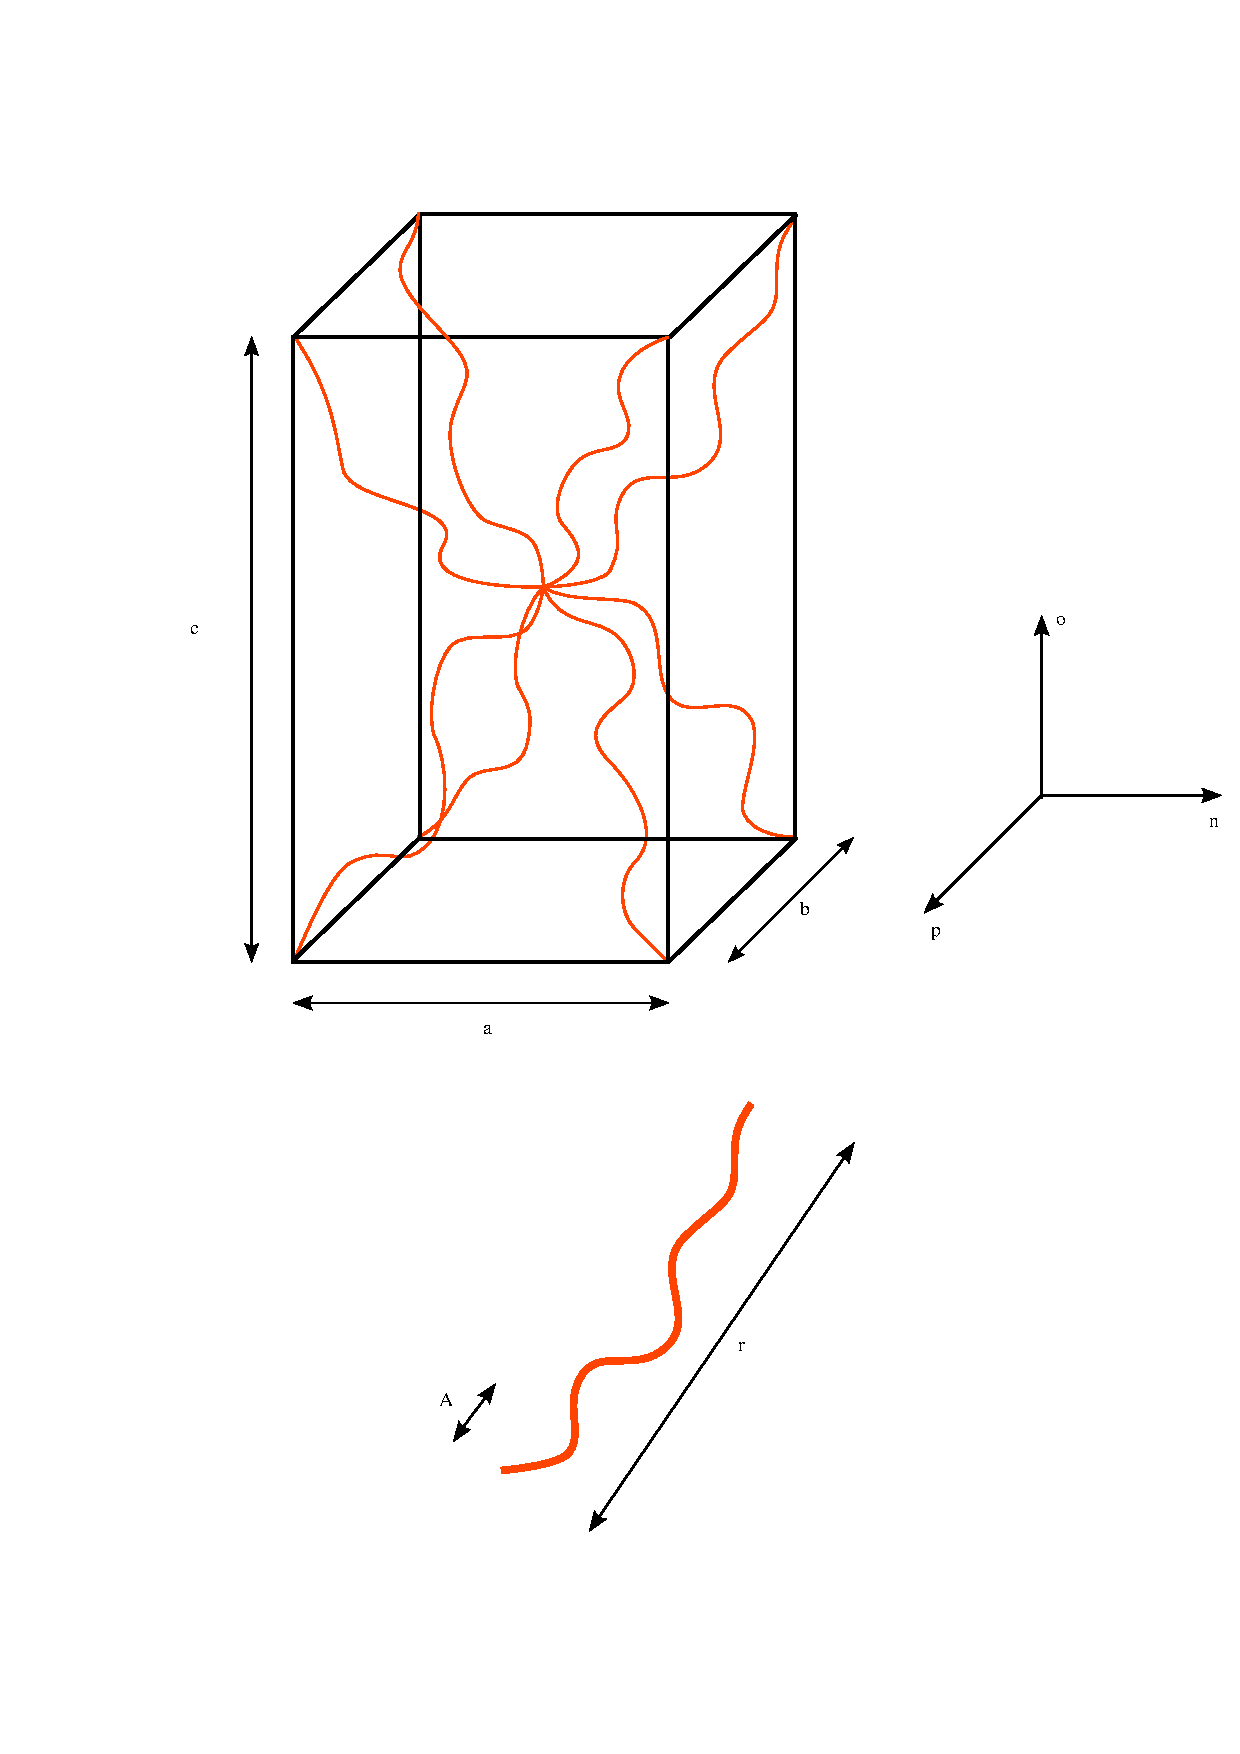
\includegraphics[width=0.8\textwidth]{images/elucidation/wlcm-cuboid}
  \caption{The eight-chain model incorporating worm-like chains.}
  \label{eight-chain-model}
\end{figure}

The elastic stretches along the unit cell axes are, respectively,
denoted by $\lambda_1^{\mathrm{e}}, \lambda_2^{\mathrm{e}}$ and
$\lambda_3^{\mathrm{e}}$, and $\bC^{\mathrm{e}^{\mathrm{c}}} =
\bF^{\mathrm{e}^{\mathrm{c}^{\mathrm{T}}}}
\bF^{\mathrm{e}^{\mathrm{c}}}$ is the elastic right Cauchy-Green
tensor of collagen. The factors $\gamma$ and $\beta$ control the bulk
compressibility of the model. The end to end chain length is given by
$r = \frac{1}{2}\sqrt{a^2\lambda_1^{\mathrm{e}^2} +
  b^2\lambda_2^{\mathrm{e}^2}+c^2\lambda_3^{\mathrm{e}^2}}$, where
$\lambda^\mathrm{e}_I =
\sqrt{\bN_I\cdot\bC^{\mathrm{e}^{\mathrm{c}}}\bN_I}$, and $\bN_I,\,I =
1,2,3$ are the unit vectors along the three unit cell axes,
respectively.

\subsection{A nearly incompressible ideal fluid}
\label{ideal-incompressible-fluid}

In this work, the fluid phase is treated as nearly incompressible and
ideal, i.e., inviscid. The partial Cauchy stress in the fluid is

\begin{equation}
\Bsigma^\mathrm{f} =
\mathrm{det}(\bF^{\mathrm{e}^\mathrm{f}})^{-1}
\bP^{\,\mathrm{f}}\bF^{\mathrm{e}^\mathrm{fT}} 
= h(\rho^\mathrm{f}){\bf 1},\label{Pf}
\end{equation}

\noindent where a large value of $h^\prime(\rho^\mathrm{f})$ ensures
near-in\-comp\-ress\-i\-bil\-i\-ty.

\subsubsection{Response of the fluid in tension; cavitation}
\label{caviation-under-tension}

The response of an ideal fluid, as defined by \mbox{Equation
  (\ref{Pf})}, does not distinguish between tension and compression,
i.e., whether $\mathrm{det}(\bF^{\mathrm{e}^\mathrm{f}}) \gtreqless
1$. Being (nearly) incompressible, the fluid can develop compressive
hydrostatic stress without bound---a case that is modelled
accurately. However, the fluid can develop at most a small tensile
hydrostatic stress \citep{cavitationchris},\footnote{Where, we are
  referring to the fluid being subject to net tension, not just a
  reduction in fluid compressive stress from reference ambient
  pressure.} and the tensile stiffness is mainly from the collagen
phase. This is not accurately represented by (\ref{Pf}), which models
a symmetric response in tension and compression.

Here, we preclude all tensile load carrying by the fluid by limiting
$\mathrm{det}(\bF^{\mathrm{e}^\mathrm{f}}) \leq 1$. We first introduce
an additional component to the relation between 
deformation of the pore space, given by $\bF$, the fluid
stress-determining tensor, 
$\bF^{\mathrm{e}^\mathrm{f}}$ and the growth tensor for the fluid,
$\bF^{\mathrm{g}^\mathrm{f}}$. Consider the cavitation (void forming) tensor,
$\bF^{\mathrm{v}}$, defined by
  
\begin{equation}
 \bF^{\mathrm{e}^\mathrm{f}}\bF^{\mathrm{g}^\mathrm{f}}
 \bF^{\mathrm{v}} = \bF.
\label{fvoid}
\end{equation}

We restrict the formulation to include only saturated current
configurations at $t = 0$. Following Section
\ref{saturation-and-tissue-swelling} we have $\tilde{v}^\mathrm{f} +
\tilde{v}^\mathrm{c} = 1$ at $t = 0$, the saturation condition in
$\Omega_t$ when solutes are at low concentrations. At times $t > 0$
Equation (\ref{saturation}) holds for
$\bF^{\mathrm{g}^\mathrm{f}}$. If
$\mathrm{det}[\bF(\bF^{\mathrm{g}^\mathrm{f}})^{-1}] \le 1$ we set
$\bF^{\mathrm{e}^\mathrm{f}} = \bF(\bF^{\mathrm{g}^\mathrm{f}})^{-1}$
and $\bF^{\mathrm{v}} = {\bf 1}$ for no cavitation. Otherwise, since
$\mathrm{det}[\bF(\bF^{\mathrm{g}^\mathrm{f}})^{-1}] > 1$, we specify
$\bF^{\mathrm{e}^\mathrm{f}} =
\mathrm{det}[\bF(\bF^{\mathrm{g}^\mathrm{f}})^{-1}]^{-1/3}\bF
(\bF^{\mathrm{g}^\mathrm{f}})^{-1}$ 
thus restricting $\bF^{\mathrm{e}^\mathrm{f}}$ to be unimodular and
allow cavitation by writing $\bF^{\mathrm{v}} =
\bF(\bF^{\mathrm{e}^\mathrm{f}}\bF^{\mathrm{g}^\mathrm{f}})^{-1}$.
These conditional relations are summarised as

\begin{equation}
\bF^{\mathrm{e}^\mathrm{f}} = \left\{ \begin{array}{ll}
  \bF(\bF^{\mathrm{g}^\mathrm{f}})^{-1},\; \bF^{\mathrm{v}} = {\bf 1},&
 \mathrm{det}[\bF(\bF^{\mathrm{g}^\mathrm{f}})^{-1}] \le 1\\
  \mathrm{det}[\bF(\bF^{\mathrm{g}^\mathrm{f}})^{-1}]^{-1/3}
  \bF(\bF^{\mathrm{g}^\mathrm{f}})^{-1}, 
  & \\
  \qquad\qquad \bF^{\mathrm{v}} =
  \bF(\bF^{\mathrm{e}^\mathrm{f}}\bF^{\mathrm{g}^\mathrm{f}})^{-1} 
  & \mathrm{otherwise.}
\end{array}\right.
\label{cavitation}
\end{equation}

\subsection{Driving forces for fluid flux}
\label{fluid-flux-constitutive-relationships}

Returning to the constitutive relation for species flux
(\ref{constitutive-relation-flux}), we first recognise that $\bM^\iota
= \rho_0^\iota\bF^{-1}\bV^\iota$ is an implicit relation for
$\bV^\iota$. Rewriting this instead as an explicit one for
$\rho^\iota_0\bV^\iota$ we have,

\begin{eqnarray}
\rho^\iota_0\bV^\iota =& &\left(\bone +
\frac{\tilde{\bD}^\iota\mathrm{GRAD}\left[\bV\right]\bF^{-1}}
     {\rho^\iota_0}\right)^{-1} 
\frac{\tilde{\bD}^\iota}{\rho^\iota_0}\nonumber\\ 
& &\cdot\left(
\ \rho_0^\iota\bg + \mathrm{DIV}\left[\bP^\iota\right] -
\rho^\iota_0\bF^{-\mathrm{T}}\left(\mathrm{GRAD}\left[e^\iota\right] -
\theta\ \mathrm{GRAD}\left[\eta^\iota\right]\right)\ \right).
\nonumber
\end{eqnarray}

\noindent From this, the constitutive relationship for mass flux is
written as a product of product of a mobility tensor and a
thermodynamic driving force,

\begin{eqnarray}
\bM^\iota & &=\underbrace{\bF^{-1}\left(\bone +
\frac{\tilde{\bD}^\iota\mathrm{GRAD}\left[\bV\right]
\bF^{-1}}{\rho^\iota_0}\right)^{-1}
\frac{\tilde{\bD}^\iota}{\rho^\iota_0}\bF^{-\mathrm{T}}}_{\bD^\iota}
\nonumber\\ 
&\cdot&\underbrace{\left(\rho_0^\iota\bF^\mathrm{T}\bg +
\bF^\mathrm{T}\mathrm{DIV}\left[\bP^\iota\right] -
\rho^\iota_0\left(\mathrm{GRAD}\left[e^\iota\right] -
\theta\ \mathrm{GRAD}\left[\eta^\iota\right]\right)\right)} 
_{\boldmath{\sF}^\iota}
\label{constitutive-relation-flux-3}
\end{eqnarray}

In particular, the constitutive relation for the flux of
extra-cellular fluid relative to collagen in the reference
configuration takes the following form,

\begin{equation}
\bM^\mathrm{f} = \bD^\mathrm{f}\left(\rho_0^\mathrm{f}\bF^T\bg +
      \bF^T\mathrm{DIV}\left[\bP^{\,\mathrm{f}}\right] -
      \rho_0^\mathrm{f}\mathrm{GRAD}\left[\mu^\mathrm{f}\right]\right),
\label{fluidflux}
\end{equation}

\noindent where $\bD^\mathrm{f}$ is the positive semi-definite
mobility of the fluid, and isothermal
conditions\footnote{Additionally, this assumption allows application
  of the Legendre transformation \mbox{$\mu^\iota = e^\iota -
    \theta\eta^\iota$} to rewrite
  \mbox{$\mathrm{GRAD}\left[e^\iota\right] -
    \theta\ \mathrm{GRAD}\left[\eta^\iota\right]$} as
  $\mathrm{GRAD}\left[\mu^\iota\right]\vert_\theta$ (at uniform
  temperature), where $\mu^\iota$ is the chemical potential.} are
assumed in order to approximate the physiological ones.

Experimentally determined transport coefficients (e.g. for mouse tail
skin \citep{Swartzetal:99} and rabbit Achilles tendons
\citep{Hanetal:2000}) are used for the fluid mobility values. Recall
that the terms in the parenthesis on the right hand-side of
\mbox{Equation (\ref{fluidflux})} sum to give the total driving force
for transport. The first term is the contribution due to gravitational
acceleration. In order to maintain physiological relevance, this term
has been neglected in the following treatment. The second term arises
from stress divergence. In the case of a non-uniform partial stress,
$\bP^\iota$, there exists a thermodynamic driving force for transport
along $\bP^\iota$. For an ideal fluid, it reduces to a pressure
gradient (as detailed in Appendix~\ref{ideal-fluid-transport}),
thereby specifying that the fluid moves down a compressive pressure
gradient, which is Darcy's Law. The third term is the gradient of the
chemical potential, $\mu^\mathrm{f} = e^\mathrm{f} - \theta
\eta^\mathrm{f}$, where $e^\mathrm{f}$ is the mass-specific internal
energy, $\theta$ is temperature and $\eta^\mathrm{f}$ is the
mass-specific entropy. The entropy gradient included in this term
results in classical Fickean diffusion if only mixing entropy exists,
as discussed in the following section.

In practice, since the driving forces in (\ref{fluidflux}) originate
from different physics, it proves useful (also seen in the following
section) to rewrite (\ref{fluidflux}) as

\begin{equation}
\bM^\mathrm{f} = \bD^\mathrm{f}_{P} \bF^T\mathrm{DIV}
\left[\bP^{\,\mathrm{f}}\right] - \bD^\mathrm{f}_{\mu}
\mathrm{GRAD}\left[e^\mathrm{f} - \theta\eta^\mathrm{f}\right],
\label{splitflux}
\end{equation}

\noindent where $\bD^\mathrm{f}_{P}$ is now the permeability of the
tissue, corresponding to stress gradient-driven transport, and
$\bD^\mathrm{f}_{\mu}$ is the mobility, corresponding to transport
driven by the gradient of the chemical potential, of the fluid phase
through the porous solid.

\subsection{Saturation and Fickean diffusion}
\label{saturation-and-fickean-diffusion}

\begin{figure}
  \begin{center}
    \psfrag{A}{\small A}
    \psfrag{B}{\small B}
    \psfrag{C}{\small C}
    \psfrag{D}{\small Vacant space}
    \psfrag{E}{\small Filled space}
    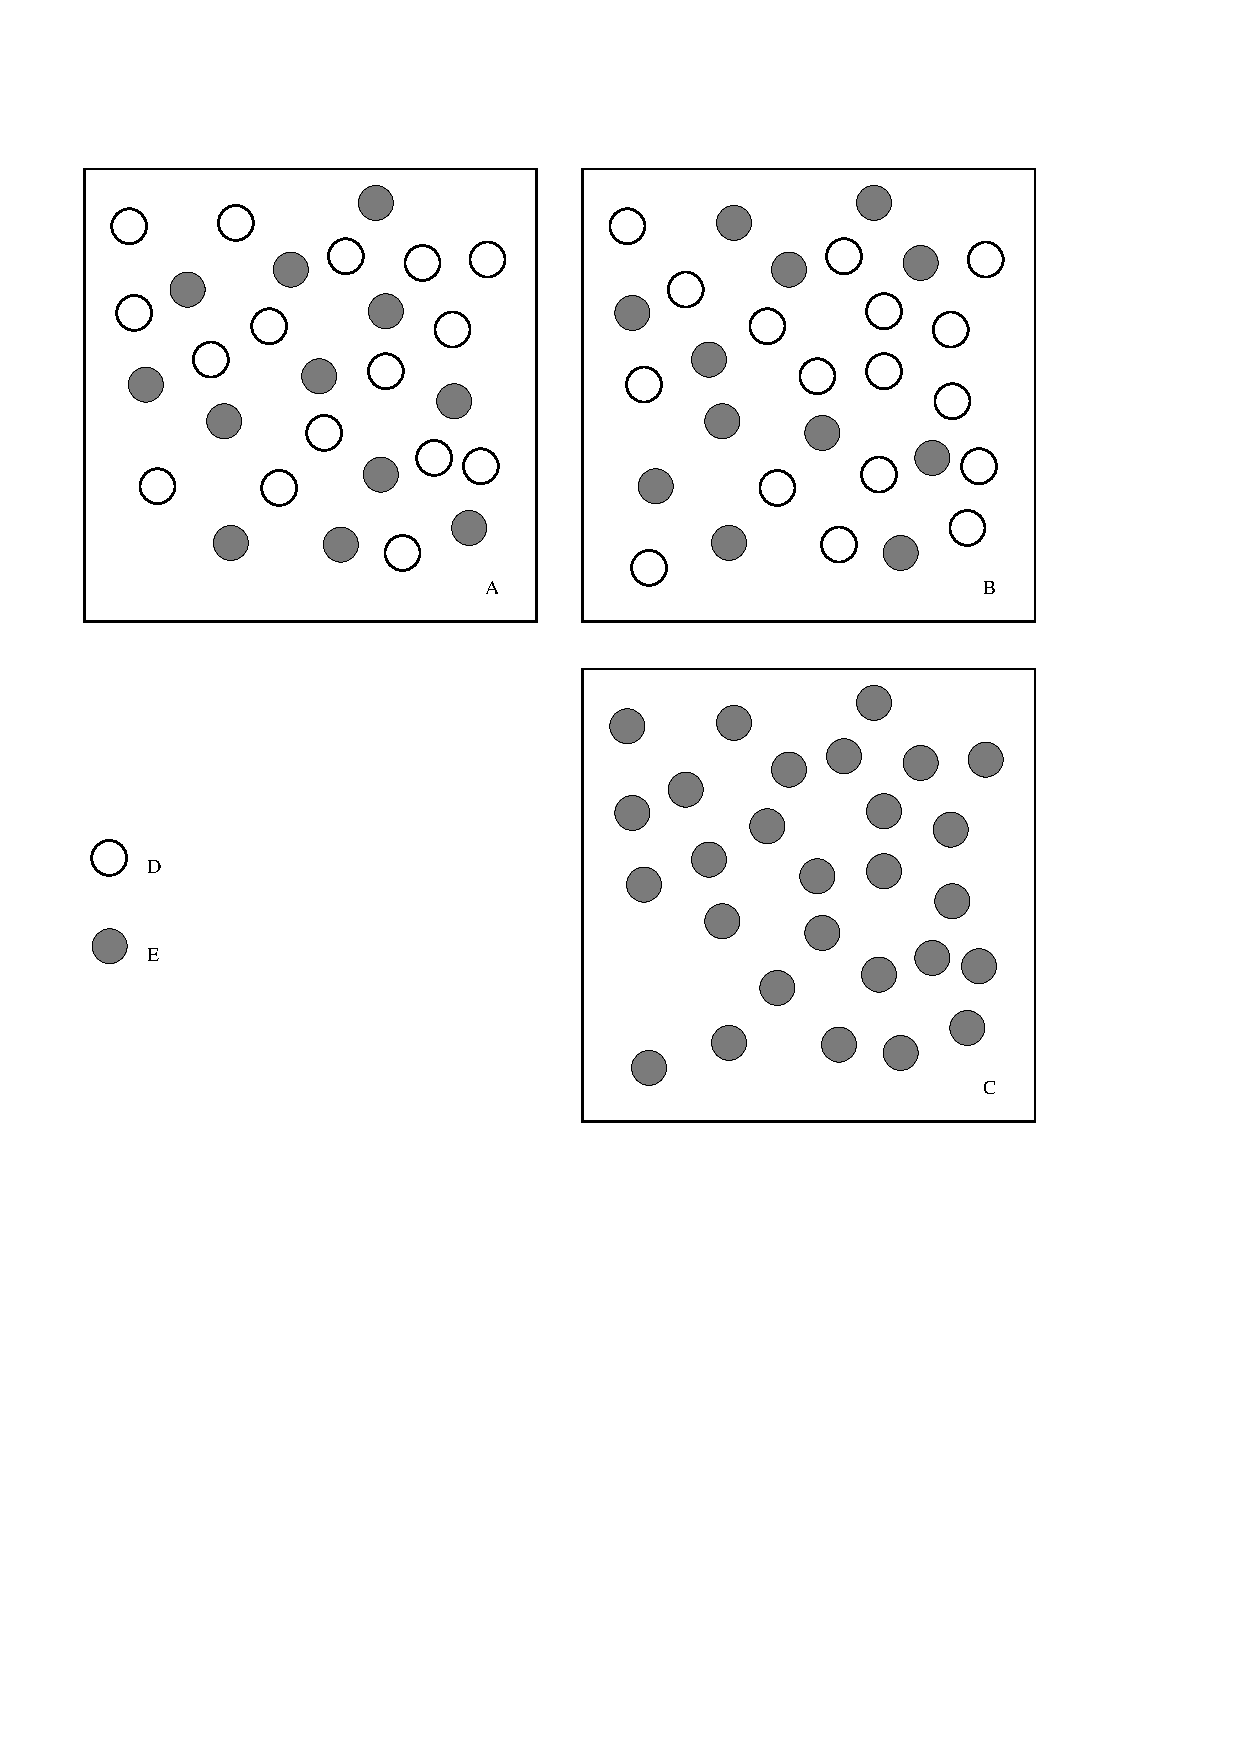
\includegraphics[width=0.8\textwidth]{images/elucidation/saturation}
    \caption{Saturation depicted at a microscopic scale}
  \end{center}
      {Depicted at a microscopic scale, only unsaturated tissues A and
        B can undergo Fickean diffusion of the fluid. C is saturated.}
      \label{fickean-diffusion}
\end{figure}

As depicted in Figure~\ref{fickean-diffusion}, only when pores are
unsaturated are there multiple configurations available to the fluid
molecules at a fixed fluid concentration.  This leads to a non-zero
mixing entropy. In contrast, if saturated, there is a single available
configuration (degeneracy), resulting in zero mixing
entropy. Consequently, Fickean diffusion, which arises from the
gradient of mixing entropy can exist only in the unsaturated
case. However, even a saturated pore structure can demonstrate
concentration gradient-dependent mass transport phenomenologically:
The fluid stress depends on fluid concentration (see Equation
(\ref{Pf})), and fluid stress gradient-driven flux appears as a
concentration gradient-driven flux.

The saturation dependence of Fickean diffusion is modelled by using
the measure of saturation introduced in
Section~\ref{saturation-and-tissue-swelling}. We rewrite the chemical
potential as

\begin{eqnarray}
\mu^\mathrm{f} &=&  
e^\mathrm{f} - \theta\eta^\mathrm{f},\ \mathrm{and}\nonumber\\
\eta^\mathrm{f} &\to& 0, \quad \mbox{as}\ \, \tilde{v}^\mathrm{f} +
\tilde{v}^\mathrm{c} \to 1.
\label{fickeanmobility}
\end{eqnarray}

\noindent It is again important to note that under physiological
conditions, soft tissues are fully saturated by fluid, and it is
appropriate to set $\mu^\mathrm{f} = e^\mathrm{f}$.

\subsection{Solute transport}
\label{solute-transport}

The dissolved solute species, denoted by s, undergo long range
transport primarily by being advected by the fluid. In addition to
this, they undergo diffusive transport relative to the fluid. This
motivates an additional velocity split of the form
\mbox{$\bV^s=\widetilde{\bV^\mathrm{s}}+\bV^\mathrm{f}$}, where
$\widetilde{\bV^\mathrm{s}}$ denotes the velocity of the solute
relative to the fluid. The constitutive relation for the corresponding
flux, denoted by $\widetilde{\bM^s}$, has the following form, similar
to Equation (\ref {fluidflux}) defined for the fluid flux.

\begin{equation}
\widetilde{\bM^\mathrm{s}} = \bD^\mathrm{s}\left( -
\rho^\mathrm{s}_0\ \mathrm{GRAD}\left[e^\mathrm{s} -
  \theta\eta^\mathrm{s}\right]\right),
\label{soluteflux}
\end{equation}

\noindent where $\bD^\mathrm{s}$ is the positive semi-definite
mobility of the solute {\em relative to the fluid}, and again,
isothermal conditions are assumed to approximate the physiological
ones. Following Section \ref{balance-of-linear-momentum} there are no
stress-dependent contributions to $\widetilde{\bM^\mathrm{s}}$.

\subsection{Nature of the sources}
\label{nature-of-sources}

There exists a large body of literature, \citep{CowinHegedus:76,
  EpsteinMaugin:2000, AmbrosiMollica:2002}, that addresses growth in
biological tissue mainly based upon a single species undergoing
transport and production/annihilation. However, from a biochemical
point of view, growth in soft biological tissue is the production and
resorption of the tissue's collagen phase as a result of a complex
cascade of biochemical reactions taking place within the cells
\citep{Alberts:02}. These processes involve several species, and
additionally involve intimate coupling between mass transfer,
biochemistry and mechanics.

An example of this chemo-mechanical coupling is seen in
Figure~(\ref{implantation-strengthening}) (from the experimental work
of \citet{calveetal:07}), where the implantation of tendon-like
engineered collagenous constructs into live rats, and their
conditioning in vivo (denoted by the blue curve) leads to significant
increases in the collagen strength and stiffness (when compared to the
in vitro control in green); highlighting the importance of the
biochemical environment on the processes underlying growth.

\begin{figure}
\centering
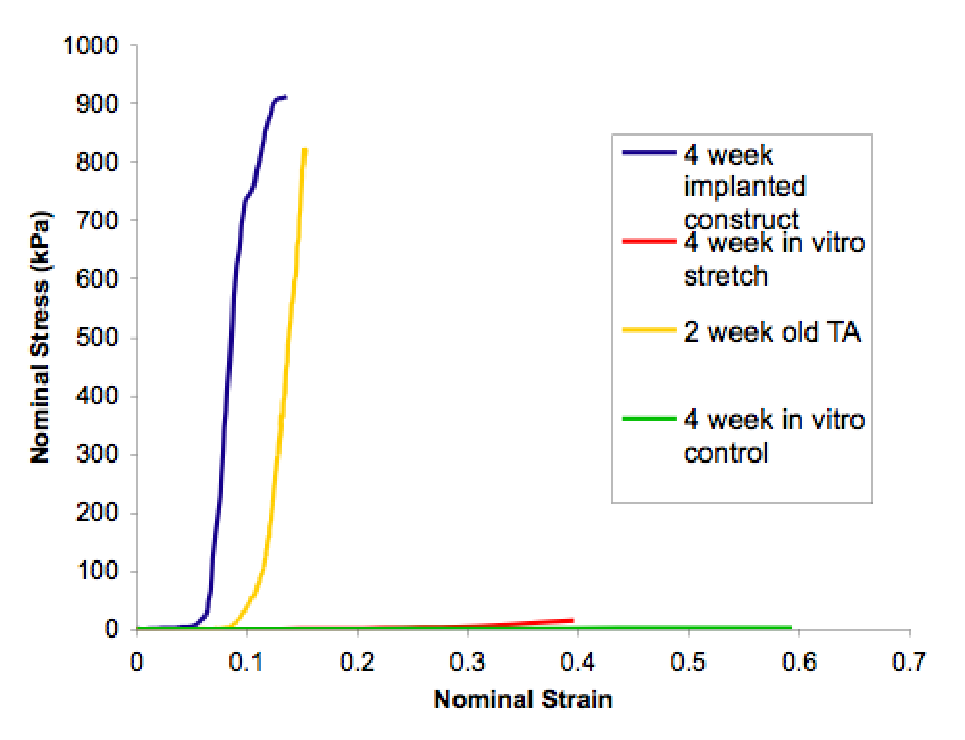
\includegraphics[width=0.8\textwidth]{images/experiments/implantation-strengthening}
\caption{Growth and strengthening of a tendon under biochemical
  influences.}
\label{implantation-strengthening}
\end{figure}

The modelling approach followed in this work is to select appropriate
functional forms of the source/sink terms, $\Pi^{\mathrm{\iota}}$,
that abstract the complexity of the biochemistry. Some specific
examples follow.

(\romannumeral 1) {\em First-order chemical kinetics} is one of the
simplest possible choices for the collagen source, and assumes that
the production of collagen is governed by a first-order rate
law. Newly-produced collagen has proteoglycan molecules bound to it,
and they in turn bind water. This effect is modelled by associating a
loss of nutrient-bearing free fluid with collagen production. A fluid
sink $\Pi^\mathrm{f}$ is introduced following first order kinetics,

\begin{equation}
\Pi^\mathrm{f} = -k^\mathrm{f}(\rho_0^\mathrm{f} -
\rho_{0_\mathrm{ini}}^\mathrm{f}),
\label{first-order-chemical-kinetics-source}
\end{equation}

\noindent and the collagen source is mathematically equivalent to the
fluid sink: $\Pi^\mathrm{c} = -\Pi^\mathrm{f}$. When
$\rho_{0}^\mathrm{f} > \rho_{0_\mathrm{ini}}^\mathrm{f}$, a certain
reference value of the fluid concentration, collagen is produced.

(\romannumeral 2) {\em Michaelis-Menten} enzyme kinetics (see, for
e.g., \cite{Sengersetal:2004}), which involves a two-step reaction, 
introduces collagen and solute source terms given by

\begin{equation}
\Pi^\mathrm{s} =
    \frac{-(k_{\mathrm{max}}\rho^{\mathrm{s}})}
    {(\rho^{\mathrm{s}}_m+\rho^{\mathrm{s}})}
    \rho_{\mathrm{cell}}, \quad\Pi^\mathrm{c} = -\Pi^\mathrm{s},
\label{enzyme-kinetics-source}
\end{equation}

\noindent where $\rho_{\mathrm{cell}}$ is the concentration of
fibroblasts, $k_{\mathrm{max}}$ is the maximum value of the solute
production reaction rate constant, and $\rho^{\mathrm{s}}_m$ is half
the solute concentration corresponding to $k_{\mathrm{max}}$. For
details on the chemistry modelled by the Michaelis-Menten model, see,
for e.g., \citet{sbromadill}.

\begin{figure}
\centering
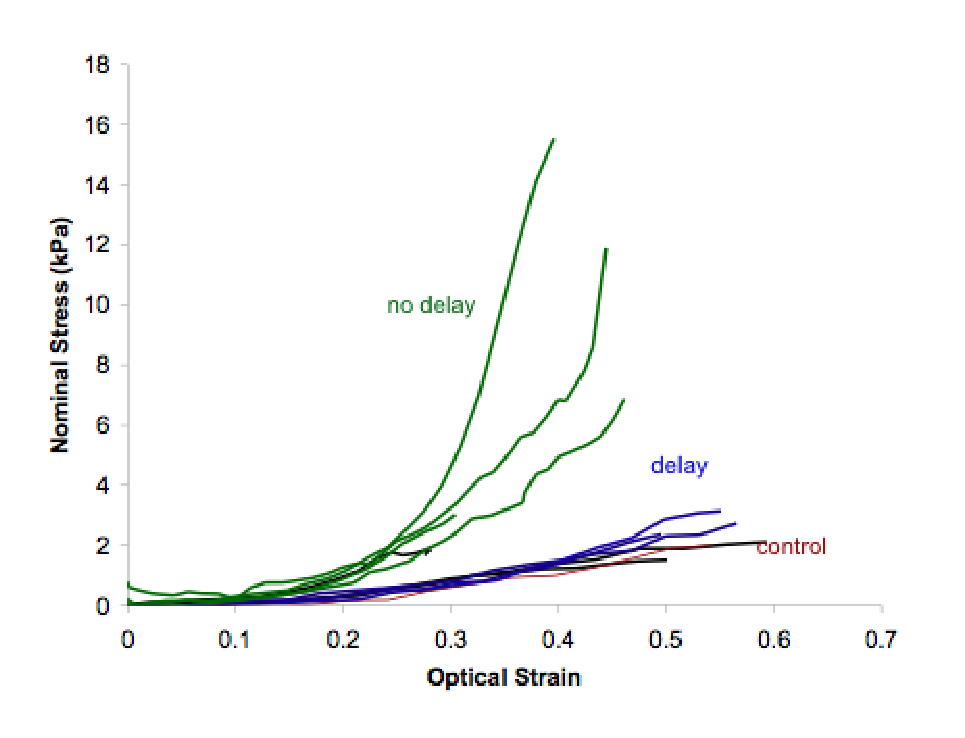
\includegraphics[width=0.8\textwidth]{images/experiments/load-strengthening}
\caption{Growth and strengthening of a tendon under mechanical
  influences.}
\label{load-strengthening}
\end{figure}

(\romannumeral 3) {\em Strain energy-dependent} sources induce growth
at a point when the energy density deviates from a reference
value. Figure~\ref{load-strengthening} (also from the experimental
work of Calve et al.) provides an example of the effect of mechanical
influences on the strengths and stiffnesses of tendons by comparing
the stress-strain responses of unloaded control specimens with those
subjected to two different load cases (denoted {\em delay} and {\em no
  delay}) on the figure.

An example of source terms of this form was originally proposed in the
context of bone growth \citep{HarriganHamilton:93}. I am not aware of
studies that have developed similar functional forms for soft tissue,
and therefore have adapted this example from the bone growth
literature, recognising that this topic is in need of further
study. Suitably weighted by a relative concentration ratio, and
written for collagen, this source term has the form

\begin{equation}
\Pi^\mathrm{c} = \left( \frac{\rho^\mathrm{c}_0}
   {\rho^\mathrm{c}_{0_\mathrm{ini}}} \right)^{-m}
   e^{\mathrm{c}}-e^{\mathrm{c}}_*,
\label{strain-energy-based-source}
\end{equation}

\noindent where $e^{\mathrm{c}}$ is the mass-specific strain energy
function of collagen, and $e^{\mathrm{c}}_*$ is a reference value of
this strain energy density. Equation
(\ref{strain-energy-based-source}) models collagen production when the
strain energy density (weighted by a concentration ratio) at a point
exceeds this reference value, and models annihilation otherwise.

\section{Algorithmic considerations}
\label{algorithmic-considerations}

Concluding the analytic formulation for biological growth presented in
this chapter, the following sections discuss some algorithmic details
that are specific to our system of interest, and underly the numerical
examples of Chapter~\ref{numerical-simulations-1}.

\subsection{The role of mass balance in the current
  configuration}
\label{role-of-current-mass-balance}

Before proceeding, we first introduce the central kinematic assumption
underlying the formulation: We assume that the pore structure deforms
with the collagenous phase. Therefore, the deformation gradient,
$\bF$, is common to c and the fluid-filled pore spaces. Furthermore,
in what follows, we will treat the fluid as ideal and
nearly-incompressible, i.e. as elastic (Section
\ref{ideal-incompressible-fluid}). This combination of kinematic and
constitutive assumptions to be elaborated upon, implies that the
stress in the fluid phase is determined by the elastic part of $\bF$
(see Sections \ref{kinematics-of-growth} and
\ref{ideal-incompressible-fluid}). For clarity we denote it as
$\bF^{\mathrm{e}^\mathrm{f}}$. Importantly, the pore-filling fluid
under stress can also undergo transport relative to the pore network;
i.e., relative to the collagenous phase. This is the fluid flux,
denoted by $\bM^\mathrm{f}$ in the reference configuration. At the
outset, we preclude stress in any of the solute species, s. Only the
solid collagen and fluid bear stress.

Although the initial/boundary value problem of mass transport can be
consistently posed in the reference configuration, the evolving
current configuration, $\Omega_t$, is of greater interest from a
physical standpoint for growth problems. It follows from the
discussion in the preceding paragraph that the shape and size of pores
in $\Omega_t$ is determined by $\bF$. Therefore, at the boundary, the
fluid concentration with respect to $\Omega_t$ remains constant if the
boundary is in contact with a fluid bath.  Accordingly, this is the
appropriate Dirichlet boundary condition to impose under normal
physiological conditions. This is shown in an idealised manner in
Figure~\ref{current-conc-fluid-bc}.

\begin{figure}
\begin{center}
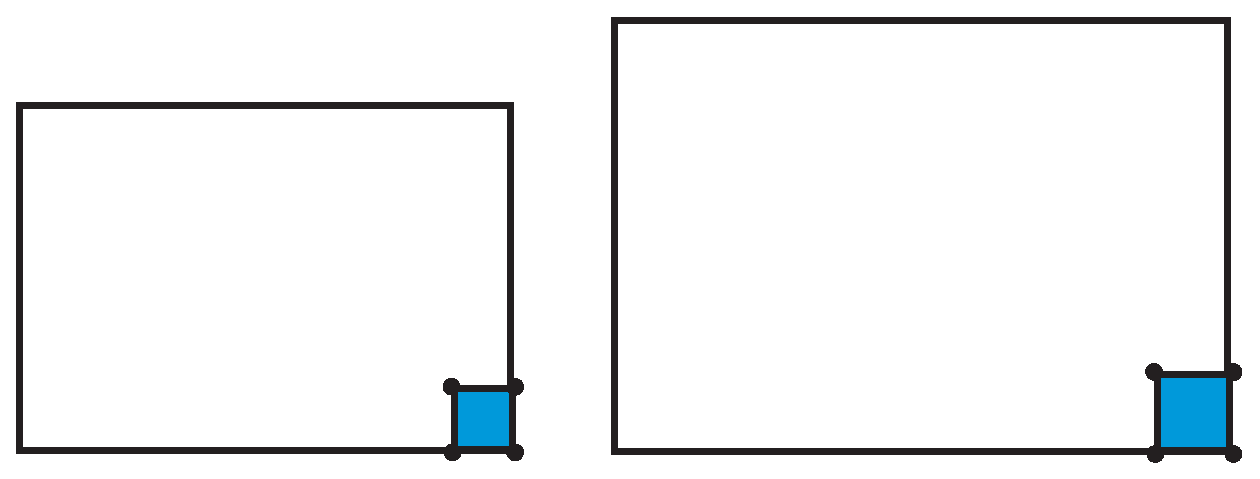
\includegraphics[width=0.8\textwidth]{images/elucidation/concentration}
\caption{Pore structure at the boundary deforming with the tissue} 
\end{center}
{If
  the pore structure at the boundary deforms with the tissue and this
  boundary is in contact with a fluid bath, the fluid concentration
  with respect to the current configuration, i.e., $\rho^\mathrm{f}$,
  remains constant.}
\label{current-conc-fluid-bc}
\end{figure}

In the interest of applying boundary conditions (either specification
of species flux or concentration) that are physically meaningful, we
use the local form of the balance of mass in the current
configuration,

\begin{equation}
\frac{\mathrm{d}\rho^\iota}{\mathrm{d}t} = \pi^\iota-
\mathrm{div}[\bm^\iota] - \rho^\iota
\mathrm{div}[\bv],\;\forall\,\iota, \label{current-mass-balance}
\end{equation}

\noindent where $\rho^\iota(\bx,t),\pi^\iota(\bx,t)$, and
$\bm^\iota(\bx,t)$ are the current mass concentration, source and mass
flux of species~$\iota$ respectively and $\bv(\bx,t)$ is the velocity
of the solid phase. They are related to corresponding reference
quantities as $\rho^\iota = \left(\mathrm{det} \left(\bF\right)
\right)^{-1} \rho_0^\iota$, $\pi^\iota = \left(\mathrm{det}
\left(\bF\right) \right)^{-1} \Pi^\iota$ and $\bm^\iota =
\left(\mathrm{det} \left(\bF\right) \right)^{-1} \bF \bM^\iota$. The
spatial divergence operator is $\mathrm{div}[\bullet]$, and
the left hand-side in Equation~(\ref{current-mass-balance}) is the material
time derivative relative to the solid, which may be written explicitly as
$\frac{\partial}{\partial t}\vert_X$, implying that the reference
position of the solid collagenous skeleton is held fixed.

\subsection{Incompressible fluid in a porous solid}
\label{incompressible-fluid-porous-solid}

Upon incorporation of the additional velocity split,
$\bV^\mathrm{s}=\widetilde{\bV^\mathrm{s}}+\bV^f$, described in
Section~\ref{solute-transport}, the resulting mass transport equation
(\ref{current-mass-balance}) for the solute species is

\begin{equation}
\frac{\mathrm{d}\rho^\mathrm{s}}{\mathrm{d}t} = \pi^\mathrm{s}-
\mathrm{div} \left[\widetilde{\bm^\mathrm{s}}+
\frac{\rho^\mathrm{s}}{\rho^f}\bm^f\right] - \rho^\mathrm{s}
\mathrm{div}[\bv].
\label{massbalcurrsol}
\end{equation}

\noindent In the hyperbolic limit, where advection dominates, spatial
oscillations emerge in numerical solutions of this equation
\citep{Brooks:82,Paper6}. However, the form in which the equation is
obtained is not in standard advection-diffusion form, and therefore is
not amenable to the application of standard stabilisation techniques
\citep{Paper6}. In part, this is because although the (near)
incompressibility of the fluid phase is embedded in the balance of
linear momentum via the fluid stress, it has not yet been explicitly
incorporated into the transport equations. This section proceeds to
impose the fluid incompressibility condition and deduces implications
for the solute mass transport equation, including a crucial
simplification allowing for its straightforward numerical
stabilisation.

From \mbox{Equation (\ref{current-mass-balance})}, the local form of
the balance of mass for the fluid species (recalling that
$\Pi^\mathrm{f}=0$) in the current configuration is

\begin{equation}
\frac{\mathrm{d}\rho^f}{\mathrm{d}t} = - \mathrm{div}\left[\bm^f\right]
- \rho^f \mathrm{div}\left[\bv\right].
\label{fluidtransporteqn}
\end{equation}

\noindent In order to impose the incompressibility of the fluid, we
first denote by $\rho_{0_{\mathrm{ini}}}^{f}$ the {\sl initial} value
of the fluid reference concentration. Recall that the fluid
concentration with respect to the reference configuration evolves in
time; $\rho^\mathrm{f}_0 = \rho^\mathrm{f}_0(\bX,t)$. Therefore we can
precisely, and non-trivially, define
$\rho_{0_{\mathrm{ini}}}^{\mathrm{f}}(\bX)$   

\begin{equation}
\begin{split}
\rho_{0}^{\mathrm{f}}(\bX,0)
                   &=:\rho_{0_{\mathrm{ini}}}^{\mathrm{f}}(\bX)\\ 
                   &=\rho_{\mathrm{ini}}^{\mathrm{f}}(\bx\circ\Bvarphi)
                   J(\bX, t)\\ &=\frac{\rho^{\mathrm{f}}
                   (\bx\circ\Bvarphi,t)} {J^{f_\mathrm{g}}(\bX,t)}
                   J(\bX,t)\\ &=\rho^{\mathrm{f}} (\bx\circ\Bvarphi,t)
                   \cancelto{\approx 1\ \forall\ t}
                   {J^{f_\mathrm{e}}}(\bX,t).\\
\label{incompderiv}
\end{split}
\end{equation}

In (\ref{incompderiv}), $J := \mathrm{det}(\bF)$ and $J^{f_\mathrm{g}} :=
\mathrm{det}(\bF^{\mathrm{g}^{\mathrm{f}}})$. The quantity
$\rho_{\mathrm{ini}}^{\mathrm{f}}$ is defined by the right hand-sides
of the first and second lines of (\ref{incompderiv}). To follow the
argument, consider, momentarily, a \emph{compressible} fluid. If the
current concentration, $\rho^\mathrm{f}$, changes due to elastic
deformation of the fluid and by transport, then
$\rho_{\mathrm{ini}}^{\mathrm{f}}$ as defined is not a
physically-realized fluid concentration. It bears a purely
mathematical relation to the current concentration, $\rho^\mathrm{f}$,
since the latter quantity represents the effect of deformation of a
tissue point as well as change in mass due to transport at that
point. If the contribution due to mass change at a point is scaled
out of $\rho^\mathrm{f}$ the quotient is identical to the result of
dividing $\rho_{0_{\mathrm{ini}}}^{\mathrm{f}}$ by the deformation
only. This is expressed in the relation between the right hand-sides
of the second and third lines of (\ref{incompderiv}). The elastic
component of fluid volume change in a pore is $J^{f_\mathrm{e}} :=
\mathrm{det}(\bF^{\mathrm{e}^{\mathrm{f}}})$, which appears  in the third
line of (\ref{incompderiv}) via the preceding arguments. Clearly then,
for a fluid demonstrating near incompressibility intrinsically (i.e.,
the true density is nearly constant), we have $J^{f_\mathrm{e}}
\approx 1$ as indicated. Equation (\ref{incompderiv}) therefore shows
that for a nearly incompressible fluid occupying the pores of a
tissue, if we further assume that the pore structure deforms as the
solid collagenous skeleton, $\rho_0^\mathrm{f}(\bX,0) \approx
\rho^\mathrm{f}(\bx\circ\Bvarphi,t)$. The fluid concentration as
measured in the current configuration is approximately constant in
space and time. This allows us to write,


\begin{equation}
\frac{\partial} {\partial t}\left(
\rho_{0_{\mathrm{ini}}}^{f}(\bX) \right) \equiv 0 \Rightarrow
\frac{\partial} {\partial t}\left(\rho^{f} (\bx\circ\Bvarphi,t)
\right)\Big\vert_{\bX} = 0,
\end{equation}

\noindent which is the hidden implication of our assumption of a
homogeneous deformation, i.e., $\bF$ is the deformation gradient of
solid collagen and the pore spaces.  This leads to $\frac{\mathrm{d}
  \rho^f} {\mathrm{d} 
  t}=0$.\footnote{Which results in a very large pressure gradient
  driven flux due to incompressibility. } We
therefore proceed to treat our fluid mass transport at steady
state. Rewriting the flux $\bm^{\mathrm{f}}$ from \mbox{Equation
(\ref{fluidtransporteqn})} as the product $\rho^{\mathrm{f}}
\bv^{\mathrm{f}}$ and using the result derived above,
\begin{equation}
\begin{split}
0 &= \left. \frac{\partial \rho^f}{\partial t} \right|_{\bX}\\ &=
-\mathrm{div}\left[\rho^f \bv^{f}\right] - \rho^f
\mathrm{div}\left[\bv\right].
\end{split}
\label{incomprimpl}
\end{equation}

\noindent Returning to (\ref{massbalcurrsol}) with this result,

\begin{equation}
\begin{split}
\frac{\mathrm{d}\rho^\mathrm{s}}{\mathrm{d}t} &= \pi^\mathrm{s}-
\mathrm{div} \left[\widetilde{\bm^\mathrm{s}}+
\frac{\rho^\mathrm{s}}{\rho^f}\bm^f\right] - \rho^\mathrm{s}
\mathrm{div}[\bv]\\ &= \frac{\rho^\mathrm{s}}{\rho^f}\left(\cancelto{0}
{-\mathrm{div}\left[\rho^f \bv^{f}\right] - \rho^f
\mathrm{div}[\bv]}\right)\\ &\quad{} + \pi^\mathrm{s} -
\mathrm{div}\left[\widetilde{\bm^\mathrm{s}}\right]
-\bm^f\cdot\mathrm{grad}\left[\frac{ \rho^\mathrm{s}}{\rho^f}\right].\\
\end{split}
\end{equation}

Thus, using the incompressibility condition (\ref{incomprimpl}), we
get the simplified form of the balance of mass for an arbitrary solute
species, s,

\begin{equation}
\frac{\mathrm{d}\rho^\mathrm{s}}{\mathrm{d}t}=\pi^\mathrm{s} -
\mathrm{div}\left[\widetilde{\bm^\mathrm{s}}\right] -
\frac{\bm^f\cdot\mathrm{grad}\left[\rho^\mathrm{s}\right]}{\rho^f} +
\frac{\rho^\mathrm{s} \bm^f \cdot \mathrm{grad}\left[\rho^f\right]}
{\rho^{f^2}}.
\label{stdform}
\end{equation}

\noindent Using the pushed-forward form of (\ref{soluteflux}), this is
now in standard advection-diffusion form, 

\begin{equation}
\begin{split}
& \frac{\mathrm{d}\rho^\mathrm{s}}{\mathrm{d}t} - \underbrace{
 \mathrm{div}\left[\bar{\bD^\mathrm{s}}\ \mathrm{grad}
 \left[ \rho^\mathrm{s}\right]\right]}_\text{Diffusion term}
 - \underbrace{\pi^\mathrm{s}}_\text{Source term} =
\\ \ & - \underbrace{\frac{\bm^f\cdot\mathrm{grad}
    \left[\rho^\mathrm{s}\right]}{\rho^f}}
_\text{Advection term} +
\underbrace{ \frac{\rho^\mathrm{s} \bm^f \cdot \mathrm{grad}\left[\rho^f\right]}
     {\rho^{f^2}},}_\text{Additional, $\rho^\mathrm{s}$-dependent source term}
\end{split}
\label{morestdform}
\end{equation}

\noindent where $\bar{\bD^\mathrm{s}}$ is a positive semi-definite
diffusivity, $\bm^{f}/\rho^{f}$ is the advective velocity, and
$\pi^\mathrm{s}$ is the volumetric source term. This form is well
suited for stabilisation schemes such as the streamline upwind
Petrov-Galerkin (SUPG) method (see, for e.g., \cite{Paper6}),
described briefly below, which limit spatial oscillations otherwise
observed when the element {\em P\'eclet number}, a measure of the
relative magnitude of advection to diffusion, is
large. Figure~\ref{unstable-solution} visually demonstrates this
oscillation for a simple advection-diffusion problem at a large
P\'eclet number.

\begin{figure}
\centering
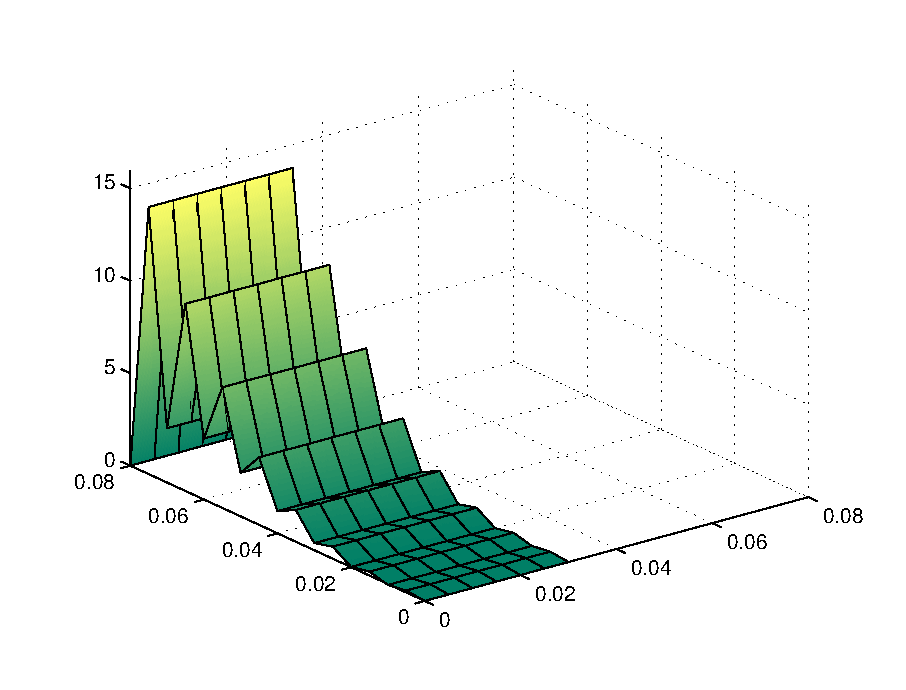
\includegraphics[width=0.8\textwidth]{images/elucidation/unstable-advection.eps}
\caption{Advection and diffusion with a P\'eclet number of $100$
  without stabilisation.}
\label{unstable-solution}
\end{figure}

\subsection{Stabilisation of the simplified solute transport equation}
\label{stabilisation-solute-transport}

\begin{figure}
\centering
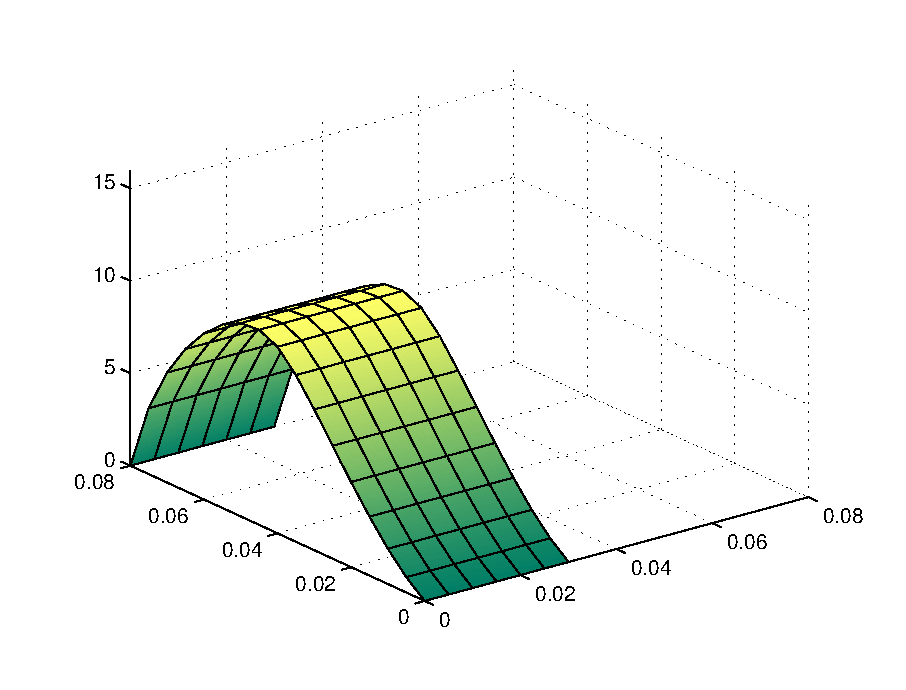
\includegraphics[width=0.8\textwidth]{images/elucidation/stable-advection.eps}
\caption{Advection and diffusion with a P\'eclet number of $100$
  with stabilisation.}
\label{stable-solution}
\end{figure}

In weak form, the SUPG-stabilised method for
Equation~(\ref{morestdform}) is

\begin{equation}
\begin{split}
&\int_{\Omega} w^{\mathrm{h}} \left(
  \frac{\mathrm{d}\rho^{\mathrm{s}^{h}}}{\mathrm{d}t} +
  \bm^f\cdot\mathrm{grad}\left[\frac{
      \rho^{\mathrm{s}^{h}}}{\rho^f}\right] \right)
  d\Omega\\ &+\int_{\Omega} \left( \mathrm{grad}
  \left[w^{\mathrm{h}}\right] \cdot \bar{\bD^\mathrm{s}} \mathrm{grad}
  \left[ \rho^{\mathrm{s}^{h}}\right] \right)\ d\Omega\\ +&
  \sum_{\mathrm{e}=1}^{\mathrm{n_{el}}} \int_{\Omega_{\mathrm{e}}}
  \tau \frac{\bm^{f}}{\rho^f} \cdot \mathrm{grad} \left[w^{\mathrm{h}}\right] \left(
  \frac{\mathrm{d}\rho^{\mathrm{s}^{h}}}{\mathrm{d}t} +
  \bm^f\cdot\mathrm{grad}\left[\frac{
      \rho^{\mathrm{s}^{h}}}{\rho^f}\right] \right) \ d\Omega\\ -&
  \sum_{\mathrm{e}=1}^{\mathrm{n_{el}}} \int_{\Omega_{\mathrm{e}}}
  \tau \frac{\bm^{f}}{\rho^f} \cdot \mathrm{grad} \left[w^{\mathrm{h}}\right]
  \left(\mathrm{div}\left[\bar{\bD^\mathrm{s}}\ \mathrm{grad} \left[
      \rho^{\mathrm{s}^{h}}\right]\right]\right) \ d\Omega\\ = &
  \int_{\Omega} w^{\mathrm{h}} \pi^\mathrm{s} \ d\Omega +
  \int_{\Gamma_{\mathrm{h}}} w^{\mathrm{h}} h \ d\Gamma\\ +&
  \sum_{\mathrm{e}=1}^{\mathrm{n_{el}}} \int_{\Omega_{\mathrm{e}}}
  \tau \frac{\bm^{f}}{\rho^f} \cdot \mathrm{grad} \left[w^{\mathrm{h}}\right]
  \pi^\mathrm{s} \ d\Omega,
\label{stabilizedmassbal}
\end{split}
\end{equation}

\noindent where quantities with the superscript $\mathrm{h}$ represent
finite-di\-men\-sion\-al approximations of infinite-dimensional field
variables, $\Gamma_{\mathrm{h}}$ is the Neumann boundary, and this
equation introduces a numerical stabilisation parameter $\tau$, which
we have calculated from the $\mathrm{L}_{2}$ norms of element level
matrices, as described in
\cite{tezduyarsupg}. Figure~\ref{stable-solution} shows the stabilised
solution for the simple advection-diffusion problem considered
previously at the same large P\'eclet number.

%

% Local Variables:
% TeX-master: "thesis"
% mode: latex
% mode: flyspell
% End:
